\documentclass[a4paper,12pt,times,twoside,custommargin,PageStyleII,numbered,print,index,fleqn]{Classes/PhDThesisPSnPDF}
\usepackage{pdfpages}

% ******************************************************************************
% ****************************** Custom Margin *********************************

% Add `custommargin' in the document class options to use this section
% Set {innerside margin / outerside margin / topmargin / bottom margin}  and
% other page dimensions
\ifsetCustomMargin
  \RequirePackage[left=35mm,right=30mm,top=35mm,bottom=30mm]{geometry} 
   \pagestyle{plain}
%\setFancyHdr % To apply fancy header after geometry package is loaded
\fi

% Add spaces between paragraphs
%\setlength{\parskip}{0.5em}
% Ragged bottom avoids extra whitespaces between paragraphs
\raggedbottom
% To remove the excess top spacing for enumeration, list and description
\usepackage{enumitem}
\setlist[enumerate,itemize,description]{noitemsep,topsep=0em}

% *****************************************************************************
% ******************* Fonts (like different typewriter fonts etc.)*************

% Add `customfont' in the document class option to use this section

\ifsetCustomFont
  % Set your custom font here and use `customfont' in options. Leave empty to
  % load computer modern font (default LaTeX font).
  %\RequirePackage{helvet}

  % For use with XeLaTeX
  %  \setmainfont[
  %    Path              = ./libertine/opentype/,
  %    Extension         = .otf,
  %    UprightFont = LinLibertine_R,
  %    BoldFont = LinLibertine_RZ, % Linux Libertine O Regular Semibold
  %    ItalicFont = LinLibertine_RI,
  %    BoldItalicFont = LinLibertine_RZI, % Linux Libertine O Regular Semibold Italic
  %  ]
  %  {libertine}
  %  % load font from system font
  %  \newfontfamily\libertinesystemfont{Linux Libertine O}
\fi

% *****************************************************************************
% **************************** Custom Packages ********************************

% ************************* Algorithms and Pseudocode **************************

%\usepackage{algpseudocode}


% ********************Captions and Hyperreferencing / URL **********************

% Captions: This makes captions of figures use a boldfaced small font.
%\RequirePackage[small,bf]{caption}

\RequirePackage[labelsep=space,tableposition=top]{caption}
\renewcommand{\figurename}{\bfseries Gambar } %to support older versions of captions.sty
\renewcommand{\tablename}{\bfseries Tabel }


% *************************** Graphics and figures *****************************

%\usepackage{rotating}
%\usepackage{wrapfig}

% Uncomment the following two lines to force Latex to place the figure.
% Use [H] when including graphics. Note 'H' instead of 'h'
%\usepackage{float}
%\restylefloat{figure}

% Subcaption package is also available in the sty folder you can use that by
% uncommenting the following line
% This is for people stuck with older versions of texlive
%\usepackage{sty/caption/subcaption}
\usepackage{subcaption}

% ********************************** Tables ************************************
\usepackage{booktabs} % For professional looking tables
\usepackage{multirow}
\usepackage[table]{xcolor}

\usepackage{multicol}
%\usepackage{longtable}
\usepackage{tabularx}


% *********************************** SI Units *********************************
\usepackage{siunitx} % use this package module for SI units

% *********************************** Disable hypens *********************************
%\usepackage[none]{hyphenat}
%\usepackage[document]{ragged2e}
\tolerance=1
\emergencystretch=\maxdimen
\hyphenpenalty=10000
\hbadness=10000

% *********************************** Listing Code *********************************
\usepackage{listings}

\usepackage{color}
\definecolor{gray}{rgb}{0.4,0.4,0.4}
\definecolor{darkblue}{rgb}{0.0,0.0,0.6}
\definecolor{cyan}{rgb}{0.0,0.6,0.6}

\lstset{
  basicstyle=\ttfamily,
  columns=fullflexible,
  showstringspaces=false,
  commentstyle=\color{gray}\upshape
}

\lstdefinelanguage{XML}
{
  morestring=[b]",
  morestring=[s]{>}{<},
  morecomment=[s]{<?}{?>},
  stringstyle=\color{black},
  identifierstyle=\color{darkblue},
  keywordstyle=\color{cyan},
  morekeywords={xmlns,version,type,annotation, folde, filename, source, database, annotation, image, flickrid, owner, name, size, width, height, depth, segmented, object, pose, truncated, difficult, bdnbox, ymin, xmin, ymax, xmax}% list your attributes here
}

% ******************************* Line Spacing *********************************

% Choose linespacing as appropriate. Default is one-half line spacing as per the
% University guidelines

%\doublespacing
%\onehalfspacing
%\singlespacing

% ******************************* Chapter heading ******************************

\renewcommand{\chaptername}{BAB}

\RequirePackage{titlesec}

\titleformat
{\chapter} % command
[display] % shape
{\bfseries\large\centering} % format
{\filcenter{\MakeUppercase{\chaptertitlename}} \thechapter} % label
{1pt} % sep
{
    \uppercase
} % before-code is code preceding the title body.
[
%\vspace{-0.5ex}%
%\rule{\textwidth}{0.3pt}
] % after-code is code following the title body.
%FORMAT ****** \titlespacing{<command>}{<left>}{<before-sep>}{<after-sep>} *****
\titlespacing{\chapter}{0pt}{0pt}{5ex}

\titleformat
{\section} % command
[hang] % shape
{\bfseries} % format
{\filright{\MakeUppercase{\thesection}} } % label
{0pt} % sep
{
    \uppercase
} % before-code is code preceding the title body.
\titlespacing{\section}{0pt}{10pt}{1pt}
%\titlespacing{\section}{0pt}{5.5ex plus 1ex minus .2ex}{4.3ex plus .2ex}

\titleformat
{\subsection} % command
[hang] % shape
{\bfseries} % format
{\filright{\thesubsection} } % label
{0pt} % sep
{
} % before-code is code preceding the title body.
\titlespacing{\subsection}{0pt}{10pt}{1pt}
%\titlespacing{\subsection}{0pt}{5.5ex plus 1ex minus .2ex}{4.3ex plus .2ex}

\titleformat
{\subsubsection} % command
[hang] % shape
{\bfseries} % format
{\filright{\thesubsubsection} } % label
{0pt} % sep
{
} % before-code is code preceding the title body.
\titlespacing{\subsubsection}{0pt}{10pt}{1pt}
%\titlespacing{\subsubsection}{0pt}{5.5ex plus 1ex minus .2ex}{4.3ex plus .2ex}

% ************************ Caption *******************************
\usepackage[justification=centering]{caption}
\usepackage{ragged2e}
\captionsetup{belowskip=0pt,aboveskip=0pt}
%\captionsetup[table]{position=above, aboveskip=3pt, belowskip=10pt}
% ************************ Formatting / Footnote *******************************

% Don't break enumeration (etc.) across pages in an ugly manner (default 10000)
\clubpenalty=10000
\widowpenalty=10000

%\usepackage[perpage]{footmisc} %Range of footnote options


% *****************************************************************************
% *************************** Bibliography  and References ********************

%\usepackage{cleveref} %Referencing without need to explicitly state fig /table

% Add `custombib' in the document class option to use this section
\ifuseCustomBib
   \RequirePackage[square, sort, numbers, authoryear]{natbib} % CustomBib

% If you would like to use biblatex for your reference management, as opposed to the default `natbibpackage` pass the option `custombib` in the document class. Comment out the previous line to make sure you don't load the natbib package. Uncomment the following lines and specify the location of references.bib file

%\RequirePackage[backend=biber, style=numeric-comp, citestyle=numeric, sorting=nty, natbib=true]{biblatex}
%\bibliography{References/references} %Location of references.bib only for biblatex

\fi
\usepackage{pdfpages}
% changes the default name `Bibliography` -> `References'
\renewcommand{\bibname}{DAFTAR PUSTAKA}
\makeatletter
\renewcommand{\@biblabel}[1]{[#1]}
\AtBeginDocument{%
  \renewcommand\@bibsetup[1]{%
    \setlength{\leftmargin}{18pt}%
    \setlength{\itemindent}{0em}%
    \setlength{\itemsep}{\bibsep}%
    \setlength{\parsep}{\z@}%
  }%
}
\makeatother
% ******************************************************************************
% ************************* User Defined Commands ******************************
% ******************************************************************************

% *********** To change the name of Table of Contents / LOF and LOT ************

%\renewcommand{\contentsname}{My Table of Contents}
%\renewcommand{\listfigurename}{My List of Figures}
%\renewcommand{\listtablename}{My List of Tables}

\renewcommand{\contentsname}{DAFTAR ISI}
\renewcommand{\listfigurename}{DAFTAR GAMBAR}
\renewcommand{\listtablename}{DAFTAR TABEL}


% ********************** TOC depth and numbering depth *************************

\setcounter{secnumdepth}{3}
\setcounter{tocdepth}{2}


% ******************************* Nomenclature *********************************

% To change the name of the Nomenclature section, uncomment the following line

%\renewcommand{\nomname}{Symbols}
\renewcommand{\nomname}{Daftar Simbol}


% ********************************* Appendix ***********************************

% The default value of both \appendixtocname and \appendixpagename is `Appendices'. These names can all be changed via:

\renewcommand{\appendixtocname}{Daftar Lampiran}
\renewcommand{\appendixname}{Lampiran}

% *********************** Configure Draft Mode **********************************

% Uncomment to disable figures in `draft'
%\setkeys{Gin}{draft=true}  % set draft to false to enable figures in `draft'

% These options are active only during the draft mode
% Default text is "Draft"
%\SetDraftText{DRAFT}

% Default Watermark location is top. Location (top/bottom)
%\SetDraftWMPosition{bottom}

% Draft Version - default is v1.0
%\SetDraftVersion{v1.1}

% Draft Text grayscale value (should be between 0-black and 1-white)
% Default value is 0.75
%\SetDraftGrayScale{0.8}


% ******************************** Todo Notes **********************************
%% Uncomment the following lines to have todonotes.
%\ifsetDraft
%	\usepackage[colorinlistoftodos]{todonotes}
%	\newcommand{\mynote}[1]{\todo[author=kks32,size=\small,inline,color=green!40]{#1}}
%\else
%	\newcommand{\mynote}[1]{}
%	\newcommand{\listoftodos}{}
%\fi

% Example todo: \mynote{Hey! I have a note}

% ************************ Thesis Information & Meta-data **********************
%% The title of the thesis
\title{Writing your PhD thesis in \texorpdfstring{\\ \LaTeX2e}{LaTeX2e}}
%\texorpdfstring is used for PDF metadata. Usage:
%\texorpdfstring{LaTeX_Version}{PDF Version (non-latex)} eg.,
%\texorpdfstring{$sigma$}{sigma}

%% Subtitle (Optional)
% \subtitle{}

%% The full name of the author
\author{Tegar Imansyah}

%% Department (eg. Department of Engineering, Maths, Physics)
\dept{PROGRAM STUDI TEKNIK MEKATRONIKA}

%% University and Crest
\university{POLITEKNIK ELEKTRONIKA NEGERI SURABAYA}
% Crest minimum should be 30mm.
\crest{\includegraphics[width=0.4\textwidth]{University_Crest}}
%% Use this crest, if you are using the college crest
%% Crest long miminum should be 65mm
%\crest{\includegraphics[width=0.45\textwidth]{University_Crest_Long}}

%% College shield [optional] 
% Crest minimum should be 30mm.
%\collegeshield{\includegraphics[width=0.2\textwidth]{CollegeShields/Kings}}


%% Supervisor (optional)
%% for multiple supervisors, append each supervisor with the \newline command
\supervisor{
Dr.Eng. Indra Adji S, S.T., M.Eng\\
NIP 1234567890\\
Anhar Risnumawan, S.ST., M.CS\\
NIP 1234567890}

%% Supervisor Role (optional) - Supervisor (default) or advisor
\supervisorrole{\textbf{Dosen Pembimbing: }}
%% if no title is desired:
% \supervisorrole{}

%% Supervisor line width: required to align supervisors
%\supervisorlinewidth{0.35\textwidth}

%% Advisor (optional)
%% for multiple advisors, append each advisor with the \newline command
%\advisor{Dr. A. Advisor\newline
%Dr. B. Advisor}
     
%% Advisor Role (optional) - Advisor (default) or leave empty
% \advisorrole{Advisors: }
%% if no title is required
% \advisorrole{}

%% Advisor line width: required to align supervisors
%\advisorlinewidth{0.25\textwidth}


%% You can redefine the submission text:
% Default as per the University guidelines:
% ``This dissertation is submitted for the degree of''
%\renewcommand{\submissiontext}{change the default text here if needed}

%% Full title of the Degree
\degreetitle{Diploma 4}

%% College affiliation (optional)
\college{PENS college}

%% Submission date
% Default is set as {\monthname[\the\month]\space\the\year}
%\degreedate{September 2014} 

%% Meta information
\subject{LaTeX} \keywords{{LaTeX} {Thesis D4} {Mekatronika} {Politeknik Elektronika Negeri Surabaya}}


%\makeatletter
%\renewcommand{\@biblabel}[1]{[#1]}
%\AtBeginDocument{%
%  \renewcommand\@bibsetup[1]{%
%    \setlength{\leftmargin}{18pt}%
%    \setlength{\itemindent}{0em}%
%    \setlength{\itemsep}{\bibsep}%
%    \setlength{\parsep}{\z@}%
%  }%
%}
%\makeatother



\begin{document}
\begin{Cover}

\includepdf[noautoscale]{cover.pdf}
\end{Cover}

\frontmatter

%\begingroup
%\let\cleardoublepage\clearpage
%\setcounter{secnumdepth}{-1}
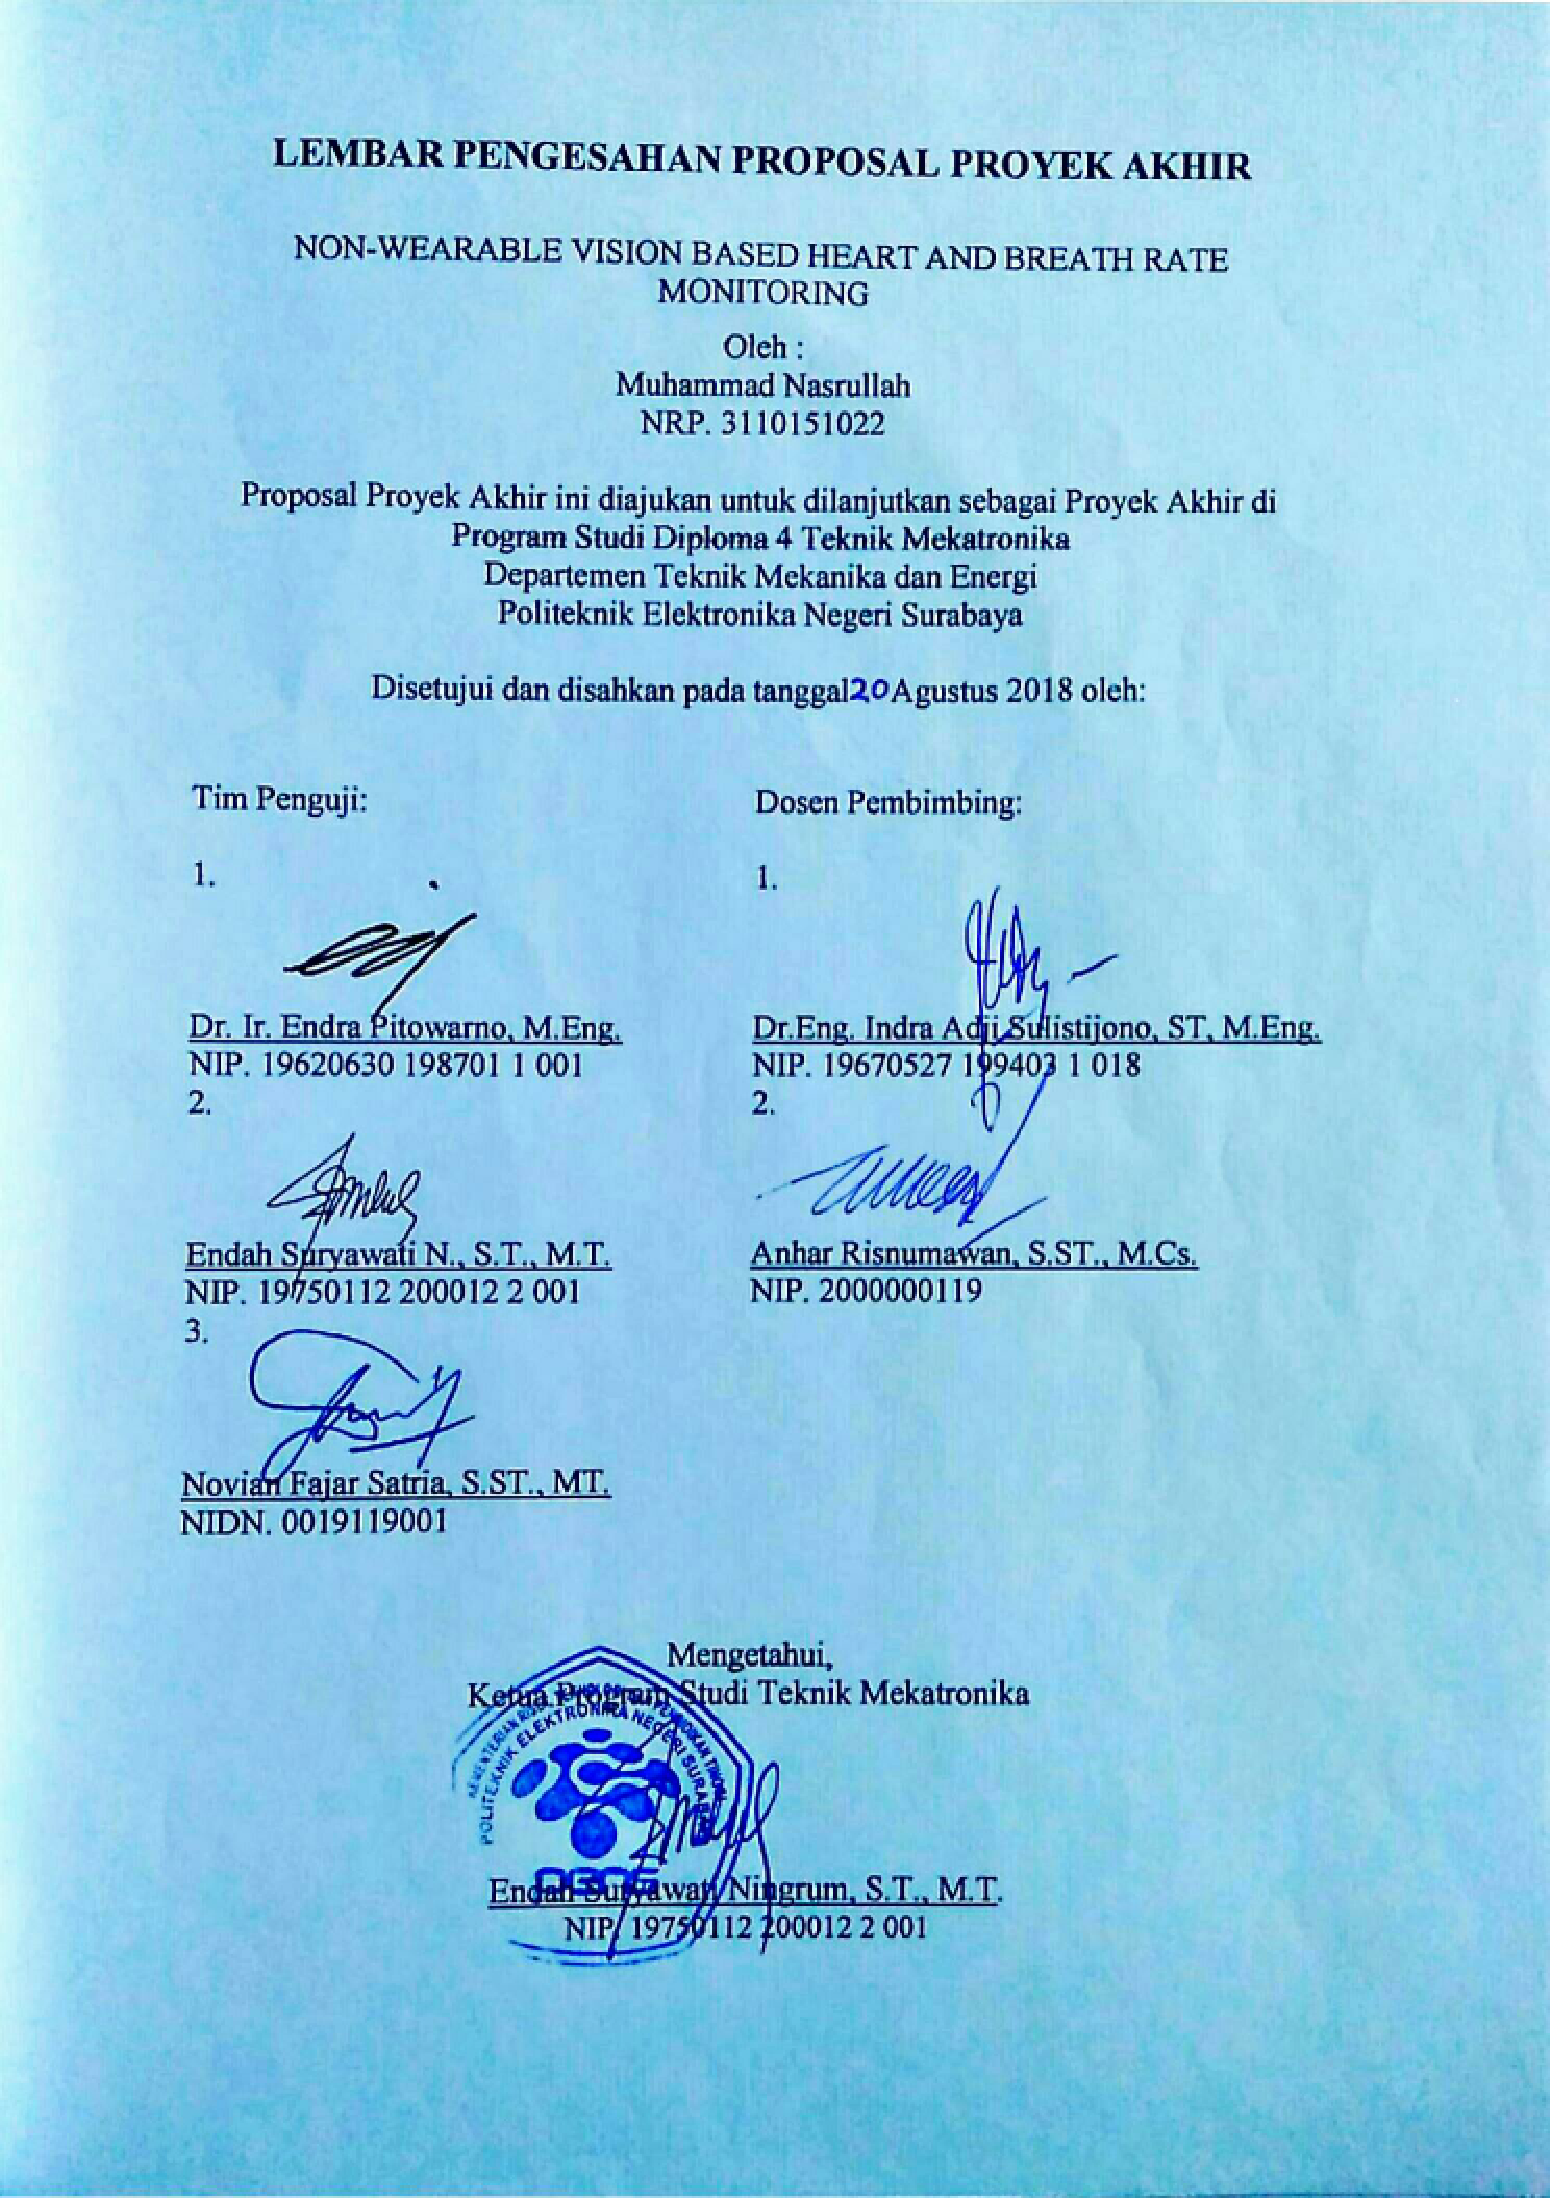
\includepdf{scan.pdf}
%% ************************** Thesis Acknowledgements **************************

\begin{acknowledgements}    

%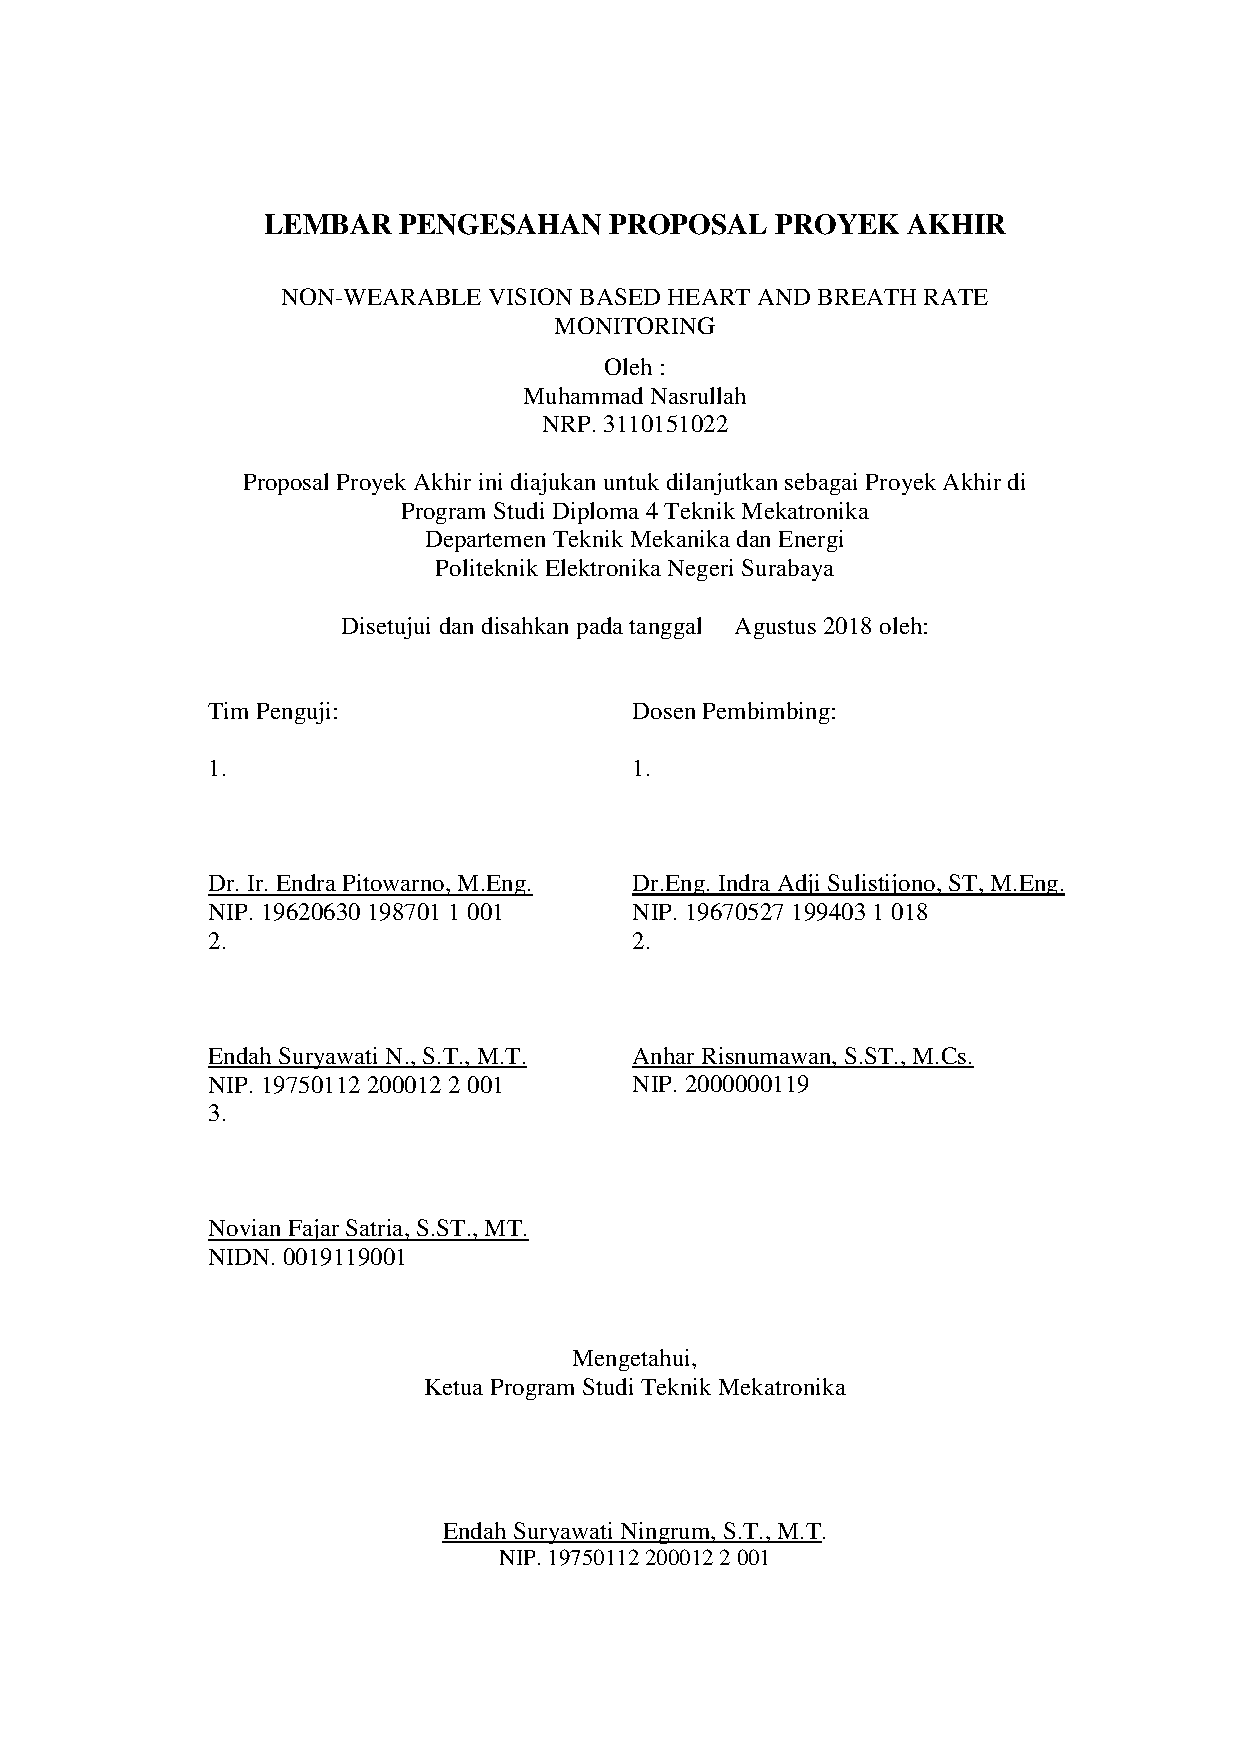
\includepdf[noautoscale]{1.pdf}
%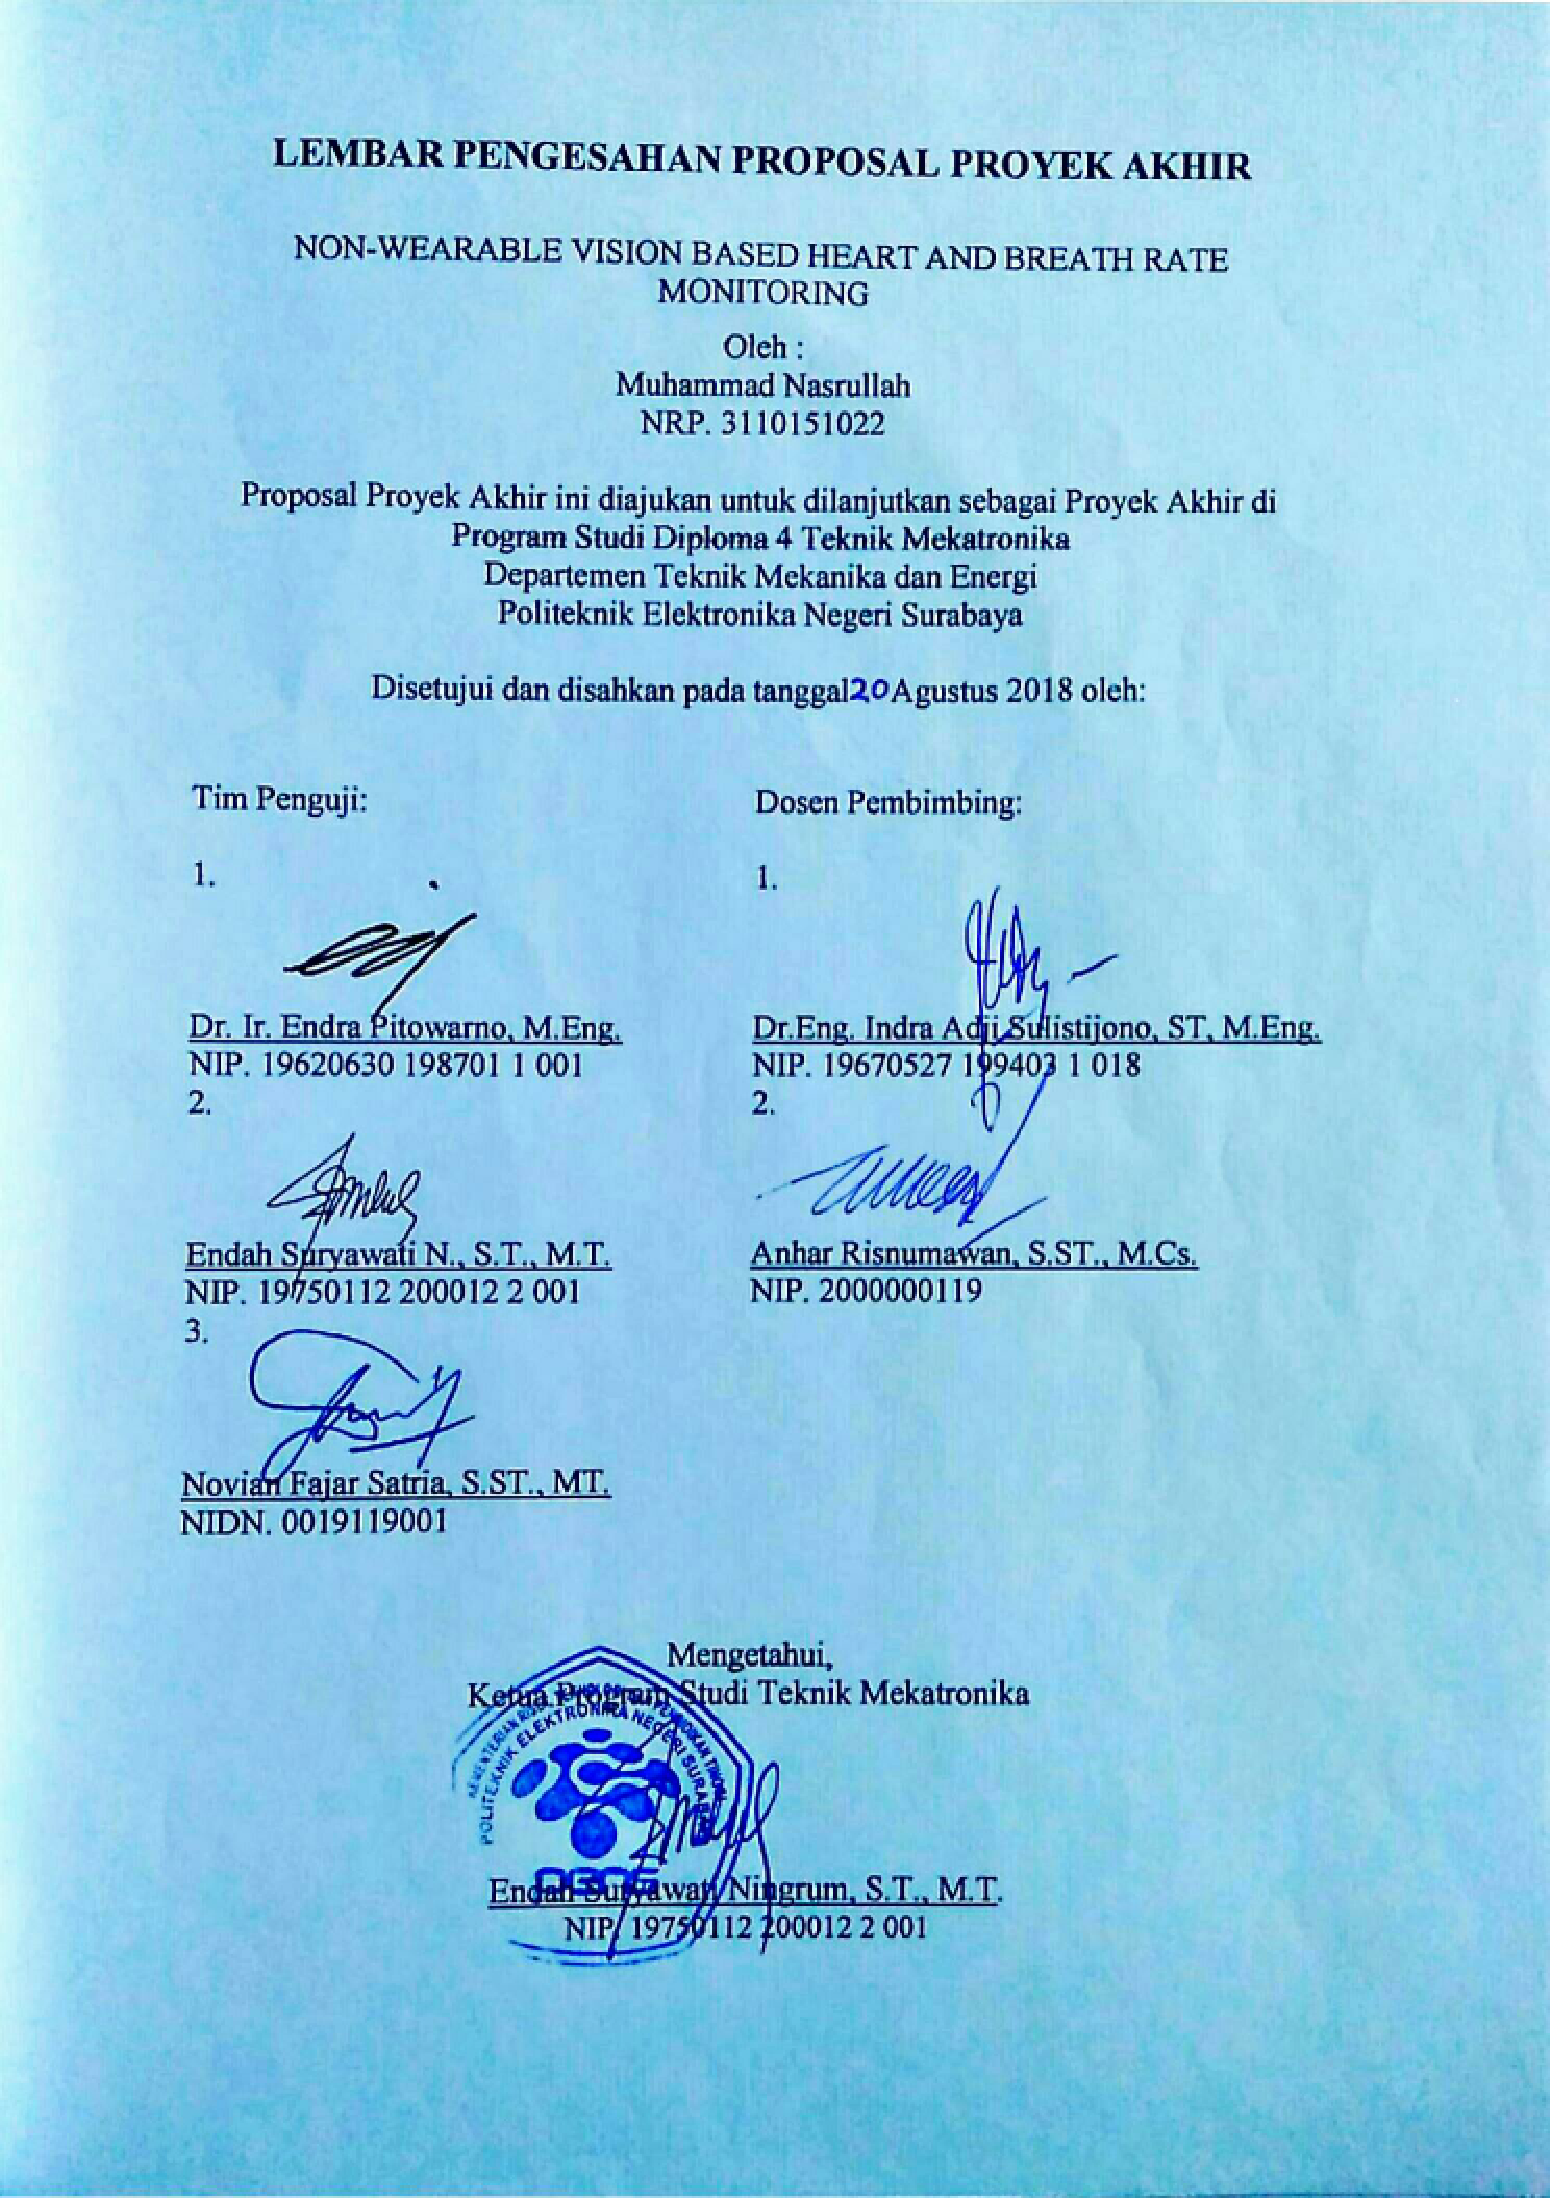
\includepdf[noautoscale]{scan.pdf}
%\addcontentsline{toc}{chapter}{Halaman Pengesahan}
\end{acknowledgements}

%\afterpage{\blankpage}
% ************************** Thesis Abstract *****************************
% Use `abstract' as an option in the document class to print only the titlepage and the abstract.
\begin{abstract}
{\setstretch{1.2}{
%Kesehatan merupakan hal yang vital bagi setiap manusia. Melakukan pengecekan kesehatan secara berkala serta antisipasi penyakit sejak dini merupakan kebutuhan yang seharunya dilakukan oleh setiap orang supaya mendapatkan rasa aman karena terhindar dari penyakit serta mendapatkan penanganan yang cepat dan tepat saat terindikasi mengidap penyakit tertentu. Namun, hal tersebut sering diabaikan oleh kebanyakan orang. Hal itu dapat disebabkan oleh beberapa faktor, diantaranya adalah minimnya sarana kesehatan di suatu daerah, proses medical check-up yang memerlukan biaya yang tidak sedikit dan membutuhkan alat bantu yang perlu dipasangkan pada pasien yang memerlukan banyak waktu serta dapat menggangu kenyamanan pasien, sehingga mereka enggan pergi ke rumah sakit atau klinik untuk melakukan pemeriksaan kesehatan jika tidak mendapati gangguan kesehatan yang mengkhawatirkan  (Pusat Data dan Informasi Kementerian Kesehatan Republik Indonesia, 2017).

Kesehatan merupakan hal yang vital bagi setiap individu. Melakukan pengecekan kesehatan secara berkala serta antisipasi penyakit sejak dini merupakan kebutuhan yang seharunya dilakukan oleh setiap orang supaya mendapatkan rasa aman karena terhindar dari penyakit serta mendapatkan penanganan yang cepat dan tepat saat terindikasi mengidap penyakit tertentu. Berdasarkan penelitian \citet{fieselmann1993}, \textit{Breathing Rate} (BR) adalah salah satu indikator tanda vital utama, dan sering digunakan untuk menyimpulkan status kesehatan kardiopulmonari subjek. Sebagai contoh, tingkat pernapasan yang lebih tinggi dari 27 kali per menit adalah prediktor paling penting untuk pasien serangan jantung. Metode yang paling umum digunakan untuk mengukur HR dan BR adalah menghitung secara manual, selain itu HR dan BR dapat diukur menggunakan berbagai sensor yang dipasangkan pada tubuh. Namun, penggunaan sensor-sensor untuk monitor HR dan BR dalam praktisnya sulit untuk diterapkan dalam kondisi tertentu karena pasien cenderung merasa tidak nyaman, misalnya pada bayi yang aktif bergerak atau ketika gerakan bebas diperlukan, diagnosa luka (luka bakar / ulkus / trauma) dan evaluasi penyembuhan kulit. Oleh karena itu, penelitian ini bertujuan untuk merancang sebuah sistem yang dapat mengukur tingkat HR dan BR tanpa diperlukan kontak langsung dengan tubuh dengan menggunakan teknik \textit{Photoplethysmography} (PPG) yang memanfaatkan pengolahan citra dan pengolahan sinyal dengan  menggunakan kerangka kerja \textit{Eulerian Video Magnification (EMV)}.

{\noindent\setstretch{1.2}\textbf{Kata Kunci:} \textit{Kesehatan, Non contact-Monitoring, \textit{Photoplethysmography} (PPG), Pengolahan Citra, Pengolahan Sinyal, Eulerian Video Magnification (EVM).}}}

\addcontentsline{toc}{chapter}{ABSTRAK}
}\end{abstract}

%\afterpage{\blankpage}
% ************************** Thesis Abstract *****************************
% Use `abstract' as an option in the document class to print only the titlepage and the abstract.
\begin{abstract_en}
{\setstretch{1.2}

\textit{Having a healthy body is an important matter for everyone. Perform a regular medical check up and early disease prevention is a necessity that should be done by each individual in order to get assurance and sense of security from a disease and also get a fast and precise treatment when indicated suffering from a certain diseases. Based on \citet{fieselmann1993}, Breathing Rate (BR) is one of the main vital sign indicators and is often used to infer subject's cardiopulmonary status. It's also reported that a respiratory rate of 27 or more was the most important predictor of cardiac arrest in hospital wards. The most commonly used method of measuring HR and BR is by manual calculaiton, in addition, HR and BR can be measured using various sensors attached to the body. However, the use of sensors for HR and BR monitoring in practice is difficult to apply under certain circumstances because the patient is likely to feel uncomfortable, for example in an active infant  or when free movement required, wound diagnosis (burn / ulcers / trauma) and evaluation of skin healing. Therefore, this study aims to design a system that can measure the level of HR and BR without direct contact with the body using \textit{Photoplethysmography} (PPG) which utilizes image processing and signal processing using \textit{Eulerian Video Magnification} (EMV) frameworks.}

{\noindent \textit{\textbf{Keywords:} Health, Non wearable Monitoring,  \textit{Photoplethysmography} (PPG), Image Processing, Signal Processing, Eulerian Video Magnification (EVM).}}


\addcontentsline{toc}{chapter}{\textit{ABSTRACT}}
}\end{abstract_en}

%\afterpage{\blankpage}
%% ******************************* Thesis Declaration ***************************

\begin{declaration}

% I hereby declare that except where specific reference is made to the work of 
% others, the contents of this dissertation are original and have not been 
% submitted in whole or in part for consideration for any other degree or 
% qualification in this, or any other university. This dissertation is my own 
% work and contains nothing which is the outcome of work done in collaboration 
% with others, except as specified in the text and Acknowledgements. This 
% dissertation contains fewer than 65,000 words including appendices, 
% bibliography, footnotes, tables and equations and has fewer than 150 figures.

Saya menyatakan bahwa tugas akhir ini berjudul \textbf{"Aerial Search and Traverse Robot (AESTRO): Deteksi Korban Bencana Alam dengan Metode Deep Learning"} merupakan hasil penelitian saya sendiri kecuali sebagaimana dikutip dalam beberapa referensi.

% Author and date will be inserted automatically from thesis.tex \author \degreedate

\end{declaration}


%% ******************************* Thesis Dedication ********************************

\begin{dedication} 

Dengan menyebut nama Allah Yang Maha Pengasih lagi Maha Penyayang, penulis menyelesaikan buku tugas akhir dengan judul:

\begin{center}
\textbf{Aerial Search and Traverse Robot (AESTRO):}
\textbf{Deteksi Korban Bencana Alam dengan Metode Deep Learning}
\end{center}

Tugas akhir ini merupakan salah satu syarat yang harus dipenuhi untuk meyelesaikan program studi Diploma 4 pada Jurusan Teknik Mekatronika Politeknik Elektronika Negeri Surabaya. Melalui kegiatan ini diharapkan mahasiswa dapat melakukan kegiatan laporan yang bersifat penelitian ilmiah dan menghubungkannya dengan teori yang telah diperoleh dalam perkuliahan. Buku ini juga disusun sepenuh hati dengan harapan pembaca mendapatkan ilmu dan gambaran dengan jelas tentang apa yang penulis kerjakan.

Pada kesempatan ini penulis panjatkan puji syukur kehadirat Allah SWT atas segala nikmat yang telah diberikan-Nya. Shalawat serta salam tidak lupa kita curahkan kepada junjungan nabi besar Nabi Muhammad SAW beserta keluarga, para sahabat dan umatnya hingga akhir zaman. Serta tidak lupa ucapan terima kasih yang sebesar-besarnya kepada beberapa pihak yang telah memberikan dukungan selama proses penyelesaian tugas akhir ini, antara lain:

\begin{enumerate}
    \item Orang tua penulis, Drs. Irwan Hermana dan Hamidah, serta seluruh keluarga besar yang selalu mengalirkan doa, memberikan semangat, nasehat, pengertian, dan dengan penuh kesabaran dalam membimbingku.
    \item Bapak Dr.Eng. Indra Adji Sulistijono, ST, M.Eng dan Anhar Risnumawan, S.ST., M.CS. selaku dosen pembimbing tugas akhir yang telah banyak membantu, membiayai dan membimbing hingga laporan ini dapat terselesaikan.
    \item Ibu Endah Suryawati Ningrum, S.T., M.T. selaku Kepala Program Studi Teknik Mekatronika PENS.
    \item Bapak dan Ibu dosen penguji tugas akhir yang telah memberikan saran dan masukannya kepada penulis.
    \item Semua Bapak dan Ibu dosen dilingkugan PENS khususnya Jurusan Teknik Mekatronika yang telah memberikan ilmu, nasehat, serta waktunya dengan ikhlas selama ini.
    \item Penghuni lab festo terutama temanku dalam tim AESTRO, Arif Dharmawan, yang berjuang bersama demi mimpinya masing masing.
    \item Teman-teman D4 Teknik Mekatronika 2013 yang luar biasa dan selalu saling menyemangati. Terutama untuk Bayu, Dimas dan Galuh atas referensi ilmu dan pengalamannya di wahana terbang.
    \item Teman-teman PENS, PENSSKY Venture, Surabaya.py dan TEDxTuguPahlawan yang telah memberi semangat, inspirasi dan kegiatan untuk melepas penat disela-sela pengerjaan tugas akhir.
    \item Serta semua pihak yang telah membantu kelancaran pelaksanaan tugas akhir yang tidak bias disebutkan satu persatu.
\end{enumerate} 

Dalam penyusunan laporan tugas akhir ini penulis menyadari akan adanya kekurangan-kekurangan baik dalam penyususnan maupun pembahasan masalah karena keterbatasan pengetahuan penulis. Untuk itu penulis mengharapkan kritik dan saran membangun dari seua pihak agar dapat lebih baik di masa yang akan datang. Terima kasih.

\end{dedication}


\tableofcontents
\listoffigures
%\afterpage{\blankpage}
\listoftables
%\endgroup


% ---------------------------

\mainmatter

%!TEX root = ../thesis.tex
%*******************************************************************************
%*********************************** First Chapter *****************************
%*******************************************************************************

\chapter{PENDAHULUAN}  %Title of the First Chapter

\ifpdf
    \graphicspath{{Chapter1/Figs/Raster/}{Chapter1/Figs/PDF/}{Chapter1/Figs/}}
\else
    \graphicspath{{Chapter1/Figs/Vector/}{Chapter1/Figs/}}
\fi


%********************************** %First Section  **************************************
\section{Latar Belakang} %Section - 1.1 


%The importance of respiratory rate is that it has been shown to be an important marker of illness and predictor of cardiac arrest.  A normal adult respiratory rate is 12-18/min.  Ventilation is carefully controlled by chemoreceptors and lung receptors and are adjusted to maintain oxygenation and rid the body of Carbon Dioxide.  Therefore any change in oxygen demand or Carbon Dioxide production will be responded to with a change in respiration.  Also any increase in acid production within the body, for example in diabetic ketoacidosis or sepsis, the respiratory rate will increase to help eliminate more Carbon Dioxide to reduce the overall level of acid within the body.

%Fieselmann et al (1993) reported that a respiratory rate of 27 or more was the most important predictor of cardiac arrest in hospital wards.  I do think that there has been an acknowledgement of this and the recording of respiratory rate is now routinely carried out and recorded.  The advent of electronic patient tracker systems requires it to be entered.

%Cretikos et al 2007 found that just over half of all patients suffering a serious adverse event on the general wards (such as a cardiac arrest or ICU admission) had a respiratory rate greater than 24 breaths/minute. Further to this they found that they could have been identified up to 24 hours before.

%\textit{Respiratory rate}(RR) berperan penting dalam mengetahui kondisi kesehatan karena telah terbukti dapat menjadi indikator penting dan prediktor serangan jantung. Tingkat pernafasan rata-rata orang dewasa normal berkisar antara 12-18 kali per menit. Pernafasan dikontrol secara hati-hati oleh kemoreseptor dan reseptor paru-paru dan disesuaikan untuk mempertahankan kadar oksigen dalam tubuh dan membuang gas karbon dioksida. Oleh karena itu setiap perubahan kebutuhan oksigen maupun produksi karbon dioksida akan direspon oleh sistem pernafasan. 

 \textit{Breathing Rate} (BR) adalah salah satu indikator tanda vital utama, dan sering digunakan untuk menyimpulkan status kesehatan kardiopulmonari subjek. Sebagai contoh, tingkat pernapasan yang lebih tinggi dari 27 kali per menit adalah prediktor paling penting untuk pasien serangan jantung [\citet{fieselmann1993}]. Berdasarkan \citet{Ganong}, rata-rata tingkat pernapasan (BR) pada orang dewasa berkisar antara 12-18 kali per menit. Kombinasi detak jantung (HR) dan tingkat pernapasan (BR) yang tinggi, tekanan darah sistolik rendah dan penurunan skor \textit{Glasgow Coma Scale} (GCS) adalah prediktor spesifik dari serangan jantung, masuk ICU yang tidak direncanakan dan kematian yang tidak terduga. Selanjutnya ditemukan bahwa kasus tersebut dapat diidentifikasi hingga 24 jam sebelum kejadian [\citet{cretikos2007}]. Berdasarkan data Badan Penelitian \citep{RI2013} dalam Gambar~\ref{fig:data_penyakit_jantung} hal tersebut akan menguntungkan pasien karena segera mendapatkan penanganan dini.

\begin{figure}[ht]
\vspace{0.5em}
\centering
 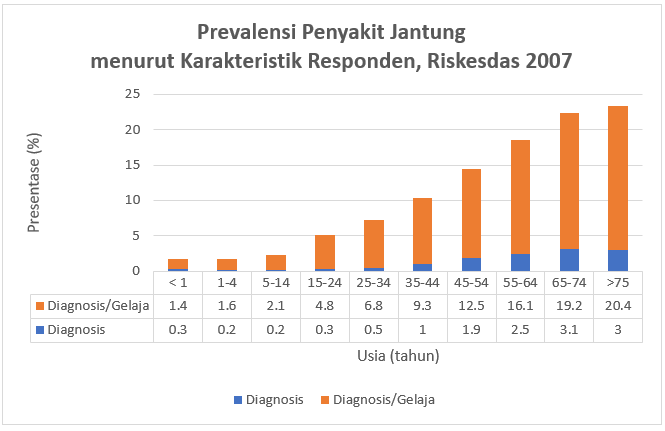
\includegraphics[width=0.7\textwidth]{chart_penderita_jantung}
 \caption{Data Penderita Penyakit Jantung Berdasarkan Rentan Usia Tahun 2007}
 \captionsetup{font={footnotesize}}
 \caption*{Sumber: Penelitian, B., 2013. Riset kesehatan dasar. Jakarta: Kementerian Kesehatan RI, halaman 116.}
 \label{fig:data_penyakit_jantung}   
\end{figure}


Pada pasien yang tidak stabil, perubahan tingkat BR relatif jauh lebih tinggi daripada perubahan nilai HR atau tekanan darah sistolik, dan dengan demikian tingkat pernapasan kemungkinan menjadi cara yang lebih baik untuk membedakan antara pasien yang stabil dan tidak [\citet{subbe2003}]. Namun, dalam kebanyakan kasus, informasi tentang HR dan BR akan mampu menunjukkan diagnosa yang lebih baik. Oleh karena itu, dalam penelitian ini sangat penting untuk mendapatkan pengukuran pasien  baik dari jantung maupun napas.


\begin{figure}[ht]
\vspace{0.5em}
\centering
\begin{subfigure}[b]{0.49\textwidth}
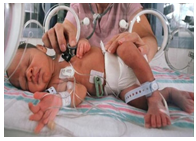
\includegraphics[width=\textwidth]{baby}
\caption{}
\end{subfigure}             
\begin{subfigure}[b]{0.49\textwidth}
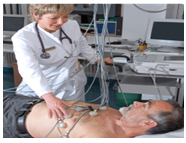
\includegraphics[width=\textwidth]{adult}
\caption{}
\end{subfigure}
\caption[Proses monitor detak jantung dan pernapasan pada bayi (a) dan orang dewasa (b)]{Proses monitor detak jantung dan pernapasan pada bayi (a) dan orang dewasa (b). Terlihat terlalu banyak selang-selang sensor yang membuat pasien tidak nyaman yang mengakibatkan posisi sensor mudah bergeser karena gerakan pasien, ataupun secara sengaja oleh pasien, khususnya pada bayi.}
\captionsetup{font={footnotesize}}
\caption*{Sumber: (a) https://www.bbc.com/news/health-30034760 \citep{Emma} (b) http://www.heart.org/HEARTORG/\\Conditions/HeartFailure/DiagnosingHeartFailure/Common-Tests-for-Heart-
Failure\_UCM\_306334\_Article.jsp \citep{web1} (diakses tanggal 6 Juni 2018)}
\label{fig:pengukuran_jantung}
\end{figure}


Penelitian sebelumnya telah diajukan dalam literatur [\citet{kristjansdottir2004,leonard2006,nilsson2000,nam2014,tarrant1997}] untuk memperkirakan nilai HR dan BR. Metode yang paling umum untuk mengukur HR dan BR adalah menghitung secara manual pergerakan jantung, dan dinding dada atau suara napas dengan stetoskop. Namun, penelitian sebelumnya telah menunjukkan bahwa metode manual ini cenderung tidak dapat diandalkan dalam perawatan pasien akut, dan dibatasi oleh keahlian pengukuran dokter [\citet{hillman2005}]. Untuk proses monitor melalui penggunaan sensor-sensor seperti \textit{Respiratory Inductance Plethysmography} (RIP), oximeter, pengukur regangan atau magnetometer telah digunakan pada penelitian-penelitian sebelumnya  [\citet{Mendelson2006,Renevey2001,tarrant1997,Yang1998}]. Photoplethysmography (PPG) juga telah banyak digunakan untuk memperkirakan tingkat pernapasan karena kesederhanaan [\citet{Allen2007,Kamal1989,kristjansdottir2004}]. Namun, penggunaan sensor-sensor untuk monitor HR dan BR dalam praktisnya sulit untuk diterapkan karena pasien cenderung merasa tidak nyaman ---khususnya pada bayi, seperti pada Gambar~\ref{fig:pengukuran_jantung}--- dan mudah mengubah posisi sensor yang berakibat pada ketidak-akuratan pengukuran.

Penelitian sebelumnya yang menggunakan \textit{non-wearable} sensor seperti kamera yaitu oleh [\citet{lazaro2014,nam2014}]. Dengan menggunakan kamera misalnya smartphone atau kamera infrared untuk memonitor HR dan BR hanya pada bagian tubuh tertentu misalnya kepala ataupun warna kulit kepala. Dalam praktisnya hal ini sulit untuk diterapkan karena metode tersebut hanya khusus untuk karakteristik bagian tubuh tertentu, dan penempatan posisi kamera terlihat kurang praktis karena menggunakan kamera sejenis smartphone.
                                          
%********************************** %Second Section  *************************************
\section{Tujuan Proyek Akhir} %Section - 1.2

Tujuan utama dari proyek akhir ini adalah mengembangkan sistem monitoring detak jantung (HR) dan pernapasan (BR) secara real-time berbasis \textit{non-wearable vision} ---menggunakan sensor yang \textit{non-wearable} berupa kamera yang tidak perlu dipasangkan langsung pada pasien---. Sistem monitoring yang dirancang tidak hanya terbatas pada bagian tubuh tertentu, namun bisa pada bagian tubuh yang lain yang menunjukkan adanya aktifitas jantung maupun pernapasan, misalnya denyut jantung pada nadi pergelangan tangan, perut, leher, dan kepala. Dengan demikian diyakini penempatan kamera akan menjadi lebih praktis misalnya dengan memanfaatkan kamera CCTV yang sudah tersedia di masing-masing kamar pasien.
Hipotesa penelitian ini adalah dengan menganalisa pergerakan piksel-piksel (RGB) pada area tubuh yang akan dimonitor HR dan BR-nya, akan didapatkan amplitudo dan frekuensi pergerakan piksel-piksel tersebut. Frekuensi dan amplitudo tertentu yang tidak kasat mata akan menggambarkan gerakan tertentu pada manusia seperti detak jantung, pernapasan, kedip mata, atau bahkan aliran darah. Piksel-piksel tersebut akan di filter sesuai frekuensi dan amplitudonya yang kemudian akan dikuatkan seperti halnya penguatan sinyal pada audio.


%********************************** % Third Section  *************************************
\section{Rumusan Masalah}  %Section - 1.3 
\label{section1.3}

Monitoring HR dan BR yang \textit{non-wearable} ---tanpa pemasangan sensor pada tubuh pasien--- sangat penting dan dibutuhkan. Pemasangan sensor-sensor pada bagian tubuh cenderung membuat tidak nyaman, dan rentan lepas atau bergeser baik itu secara sengaja ataupun tidak sengaja oleh pasien, hal ini terjadi khususnya pada bayi. Oleh karena itu, penggunaan \textit{non-wearable} sensor seperti kamera menarik untuk diteliti lebih lanjut.

Penelitian sebelumnya dengan menggunakan kamera [\citet{lazaro2014,nam2014}] cenderung fokus hanya pada bagian tubuh tertentu untuk monitor jantung dan pernapasan. Metode tertentu hanya dapat bekerja untuk bagian tubuh tertentu tetapi tidak untuk bagian tubuh lain. Ditambah dengan penggunaan kamera smartphone yang mengakibatkan kurang praktis untuk penempatan posisi kamera, misalnya di rumah sakit. Dari penjelasan sebelumnya, permasalahan yang akan dibahas dalam penelitian ini yaitu:
\begin{enumerate}
\item Apakah perbedaan pengukuran HR dan BR menggunakan metode \textit{wearable} dan \textit{non-wearable}?
\item Bagaimana proses monitoring HR dan BR menggunakan metode \textit{non-wearable}?
\item Bagaimana melakukan pengukuran HR dan BR pada bagian tubuh yang berbeda dengan menggunakan kamera?

 
\end{enumerate}

%********************************** % Forth Section  *************************************
\section{Batasan Masalah}  %Section - 1.4

Dari rumusan masalah tersebut, akan dilakukan batasan masalah yaitu:
\begin{enumerate}
 \item Pembahasan hanya mengenai proses pengolahan gambar.
 \item Monitoring dilakukan pada bagian tubuh yang menunjukkan adanya aktifitas jantung maupun pernapasan (pergelangan tangan, leher, perut dan kepala).
 \item Uji coba dilakukan pada pencahayaan yang cukup.
 \item Jarak monitoring yang terbatas.
\item Jumlah kamera yang digunakan satu.
\item Posisi kamera konstan.
\item Monitoring dilakukan selama adanya perubahan piksel.
 
\end{enumerate}

%********************************** % Fifth Section  *************************************
\section{Metodologi Proyek Akhir}  %Section - 1.5 
Metodologi yang digunakan pada penelitian tugas akhir ini adalah sebagai berikut:
\begin{enumerate}
 \item Studi Literatur
 \begin{itemize}
 \item Mencari dan mempelajari karakterisitik dan mekanisme sistem pernapasan dan detak jantung pada manusia.
    \item Mencari dan mempelajari \textit{Digital Signal Processing}.
   \item Mencari dan mengumpulkan dataset HR dan BR.
 \end{itemize}
 \item Implementasi metode untuk monitoring HR dan BR
 \begin{itemize}
 \item Proses ekstraksi sinyal HR dan BR dari bagian tubuh yang telah ditentukan.
    \item Mengolah sinyal HR dan BR yang diperoleh menjadi nilai eksak.
 \end{itemize}
\item Implementasi program 
 Berdasarkan hasil monitoring yang didapatkan sebelumnya, kemudian dibuat progam dengan \textit{User Interface} dan diaplikasikan pada hardware yang telah ditentukan untuk proses monitoring secara real time. 
 \item Proses pembuatan \textit{User Interface} program dan komunikasi serial interface.
\item Desain \textit{casing} hardware.
 \item Pengujian dan Analisa Data.
 \begin{itemize}
    \item Membahas mengenai pengujian metode dan \textit{User Interface} program dari sistem monitoring HR dan BR. 
    \item Melakukan analisa dari metode dan \textit{User Interface} program yang telah dicapai hingga saat pengujian.
 \end{itemize}
\end{enumerate}


%********************************** % Sixth Section  *************************************
\section{Sistematika Penulisan}  %Section - 1.6 

Sistematika penulisan berisi tentang bagaimana menyajikan laporan proyek akhir. Sistematika yang akan diuraikan dalam proposal proyek akhir ini terbagi dalam bab-bab yang akan dibahas sebagai berikut:
\\
BAB 1 : PENDAHULUAN

Berisi latar belakang pembuatan proyek akhir, rumusan masalah dalam proyek akhir ini, batasan masalah, tujuan dari rumusan masalah, luaran yang diharapkan, metedologi untuk menyelesaikan proyek akhir ini, dan sistematika penulisan.
\\
BAB II : STUDI PUSTAKA

Berisi tentang tinjauan pustaka penelitian sebelumnya dan teori penunjang yang mendukung dalam perencanaan serta pembuatan proyek akhir ini. Teori yang ditinjau mengacu pada penelitian-penelitian sebelumnya tentang macam-macam penelitian tentang pengukuran HR dan BR, penelitian \textit{Photoplethysmography}, dan penggunaan \textit{Digital Signal Processing}.
\\
BAB III : PERANCANGAN DAN PEMBUATAN SISTEM

Berisi tentang gambaran umum sistem yang akan dibangun, desain perancangan komputer, hardware dan komunikasi yang digunakan, serta pembuatan \textit{User Interface} program.
\\
BAB IV : PENGUJIAN DAN ANALISA SISTEM

Berisi tentang pengujian dari masing-masing bagian sistem dan pengujian sistem sementara. Pada bab ini akan diperlihatkan hasil yang telah diterapkan dan pada bagian mana dapat dilakukan penyempurnaan.
\\
BAB V : PENUTUP

Berisi kesimpulan dan analisa sistem dari proyek akhir yang telah didapat serta saran-saran untuk pengembangan selanjutnya.

% \nomenclature[z-DEM]{DEM}{Discrete Element Method}
% \nomenclature[z-FEM]{FEM}{Finite Element Method}
% \nomenclature[z-PFEM]{PFEM}{Particle Finite Element Method}
% \nomenclature[z-FVM]{FVM}{Finite Volume Method}
% \nomenclature[z-BEM]{BEM}{Boundary Element Method}
% \nomenclature[z-MPM]{MPM}{Material Point Method}
% \nomenclature[z-LBM]{LBM}{Lattice Boltzmann Method}
% \nomenclature[z-MRT]{MRT}{Multi-Relaxation 
% Time}
% \nomenclature[z-RVE]{RVE}{Representative Elemental Volume}
% \nomenclature[z-GPU]{GPU}{Graphics Processing Unit}
% \nomenclature[z-SH]{SH}{Savage Hutter}
% \nomenclature[z-CFD]{CFD}{Computational Fluid Dynamics}
% \nomenclature[z-LES]{LES}{Large Eddy Simulation}
% \nomenclature[z-FLOP]{FLOP}{Floating Point Operations}
% \nomenclature[z-ALU]{ALU}{Arithmetic Logic Unit}
% \nomenclature[z-FPU]{FPU}{Floating Point Unit}
% \nomenclature[z-SM]{SM}{Streaming Multiprocessors}
% \nomenclature[z-PCI]{PCI}{Peripheral Component Interconnect}
% \nomenclature[z-CK]{CK}{Carman - Kozeny}
% \nomenclature[z-CD]{CD}{Contact Dynamics}
% \nomenclature[z-DNS]{DNS}{Direct Numerical Simulation}
% \nomenclature[z-EFG]{EFG}{Element-Free Galerkin}
% \nomenclature[z-PIC]{PIC}{Particle-in-cell}
% \nomenclature[z-USF]{USF}{Update Stress First}
% \nomenclature[z-USL]{USL}{Update Stress Last}
% \nomenclature[s-crit]{crit}{Critical state}
% \nomenclature[z-DKT]{DKT}{Draft Kiss Tumble}
% \nomenclature[z-PPC]{PPC}{Particles per cell}
%!TEX root = ../thesis.tex
%*******************************************************************************
%****************************** Second Chapter *********************************
%*******************************************************************************

\chapter{STUDI PENDAHULUAN}

\ifpdf
    \graphicspath{{Chapter2/Figs/Raster/}{Chapter2/Figs/PDF/}{Chapter2/Figs/}}
\else
    \graphicspath{{Chapter2/Figs/Vector/}{Chapter2/Figs/}}
\fi

Elektrokardiografi (ECG atau EKG) merupakan metode standar yang paling umum digunakan dalam dunia medis untuk mengukur tingkat HR dan BR pada tubuh. Menghitung HR dan BR secara manual juga merupakan cara yang sering dilakukan. Namun, penelitian sebelumnya telah menunjukkan bahwa metode manual ini cenderung tidak dapat diandalkan dalam perawatan pasien akut, dan dibatasi oleh keahlian pengukuran dokter [\citet{hillman2005}]. Oleh karena itu, dikembangkan metode Photoplethysmography (PPG) yang memanfaatkan karakteristik gelombang cahaya untuk memonitor tingkat HR dan BR. Berdasarkan Sun dan Thakor \citep{sun2016}, metode PPG dikelompokkan menjadi dua, yaitu (a) kontak, dan (b) non-kontak. Metode PPG dengan kontak dapat disebut juga dengan istilah \textit{wearable} PPG karena prosesnya yang memerlukan kontak langsung antara sensor yang digunakan dengan bagian tubuh tertentu. Sementara itu, metode non-kontak PPG dapat disebut dengan istilah \textit{non-wearable} PPG karena tidak memerlukan kontak langsung antara sensor dengan bagian tubuh tertentu dalam prosesnya. 



%Penelitian sebelumnya untuk melakukan monitor denyut jantung (HR) dan tingkat pernapasan (BR) menggunakan sensor \textit{non-wearable} contohnya kamera \textit{Charge-Coupled Device} (CCD) [\citet{Allen2007,Estepp2014,Wu2000}], kamera RGB [\citet{deHaan2013,Mirmo2016,Poh2010,Poh2011}] serta smartphone [\citet{lazaro2014,nam2014}]. Penggunaan kamera maupun smartphone untuk memonitor HR dan BR cenderung berfokus pada bagian tubuh tertentu misalnya kepala ataupun warna kulit kepala. Dalam praktisnya hal ini sulit untuk diterapkan karena metode tersebut hanya khusus untuk karakteristik bagian tubuh tertentu, dan penempatan posisi kamera terlihat kurang praktis karena menggunakan kamera sejenis smartphone. 

\section{Karakteristik Gelombang Cahaya Pada Kulit}

\begin{figure}[ht]
	%\vspace{0.5em}
	\centering
	\includegraphics[width=0.6\textwidth]{light}
	\caption{Ilustrasi penetrasi cahaya dalam kulit.}
	\captionsetup{font={footnotesize}}  
	\caption*{sumber : https://www.researchgate.net/post/How\_depth\_low\_power\_laser\_can\_penetrate\_human\_tissue \citep{web2} (diakses tanggal 8 Agustus 2018)}
	\label{fig:light}   
\end{figure}

Interaksi antara cahaya dengan jaringan biologis bisa sangat kompleks dan mungkin melibatkan aktifitas seperti penyebaran, penyerapan dan atau pantulan cahaya. Penelitian Anderson dan Parrish \citep{ANDERSON1981} memeriksa karakteristik optis dan penetrasi cahaya pada kulit manusia. Dalam wilayah kulit yang tampak, puncak penyerapan cahaya dominan mirip dengan nilai spektrum cahaya biru, kemudian diikuti dengan wilayah spektrum cahaya hijau-kuning ---antara 500nm hingga 600nm--- yang mempunyai karakteristik mirip dengan sel darah merah. Panjang gelombang yang lebih pendek akan diserap oleh melanin. Air menyerap cahaya ultraviolet dan spektrum cahaya yang lebih panjang dari spektrum IR, sedangkan spektrum cahaya merah dan inframerah (IR) dapat dilewatkan dengan mudah. Oleh karena itu, panjang gelombang IR dapat digunakan sebagai sumber cahaya dalam sensor PPG.
Darah menyerap lebih banyak cahaya daripada jaringan tubuh lain di sekitarnya. Oleh karena itu, pengurangan jumlah darah dapat diidentifikasi sebagai peningkatan intensitas cahaya yang terdeteksi. Gambar~\ref{fig:light} menunjukkan bahwa panjang gelombang menentukan seberapa jauh penetrasi cahaya dalam kulit. Selain itu, jarak antara sumber cahaya dengan fotodetektor juga merupakan faktor yang penting. Spektrum cahaya hijau cocok digunakan untuk pengukuran aliran darah superfisial (wilayah luar) kulit. Cahaya dengan panjang gelombang antara 500 dan 600 nm menunjukkan kedalaman modulasi terbesar dengan penyerapan cahaya oleh aktifitas pulsatil darah. Panjang gelombang IR atau yang mendekati IR lebih baik untuk pengukuran aliran darah di dalam jaringan. Misalnya pengukuran aliran darah di otot. Hal tersebut membuat IR marak digunakan pada perangkat PPG selama beberapa waktu [\citet{Tamura2014}]. Namun dalam beberapa tahun terakhir penggunaan spektrum warna hijau dalam perangkat PPG semakin populer karena intensitas variasi yang besar dalam modulasi yang diamati selama siklus jantung untuk panjang gelombang hijau [Jonathan dan Leahy \citep{Enock}, \citet{Lee2013,Maeda2011,Maeda2008,Matsu2014,Scully2012}].
LED hijau memiliki daya serap yang jauh lebih besar untuk oksihemoglobin dan deoksihemoglobin dibandingkan dengan cahaya inframerah. Oleh karena itu, perubahan dalam cahaya hijau yang dipantulkan lebih besar dari pada cahaya inframerah yang dipantulkan ketika darah menembus kulit, menghasilkan rasio signal dengan gangguan yang lebih baik untuk sumber cahaya hijau [\citet{Tamura2014}].


%\section{Macam Macam Metode Pengukuran HR dan BR}
\section{Elektrokardiografi (ECG atau EKG)}

\begin{figure}[ht]
%\vspace{0.5em}
\centering
\begin{subfigure}[b]{0.49\textwidth}
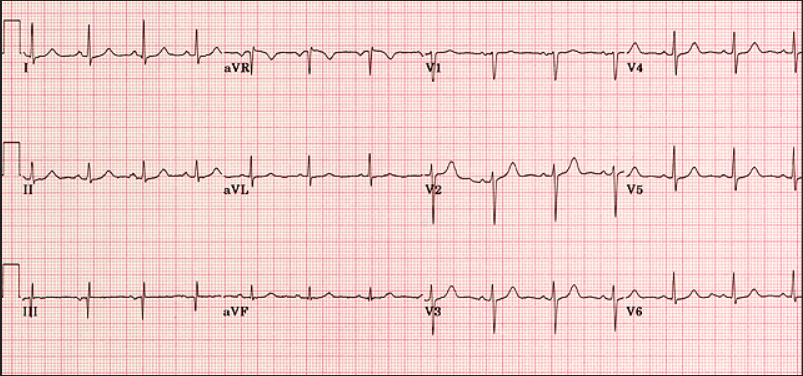
\includegraphics[width=\textwidth]{Normal_ECG}
\caption{}
\end{subfigure}             
\begin{subfigure}[b]{0.49\textwidth}
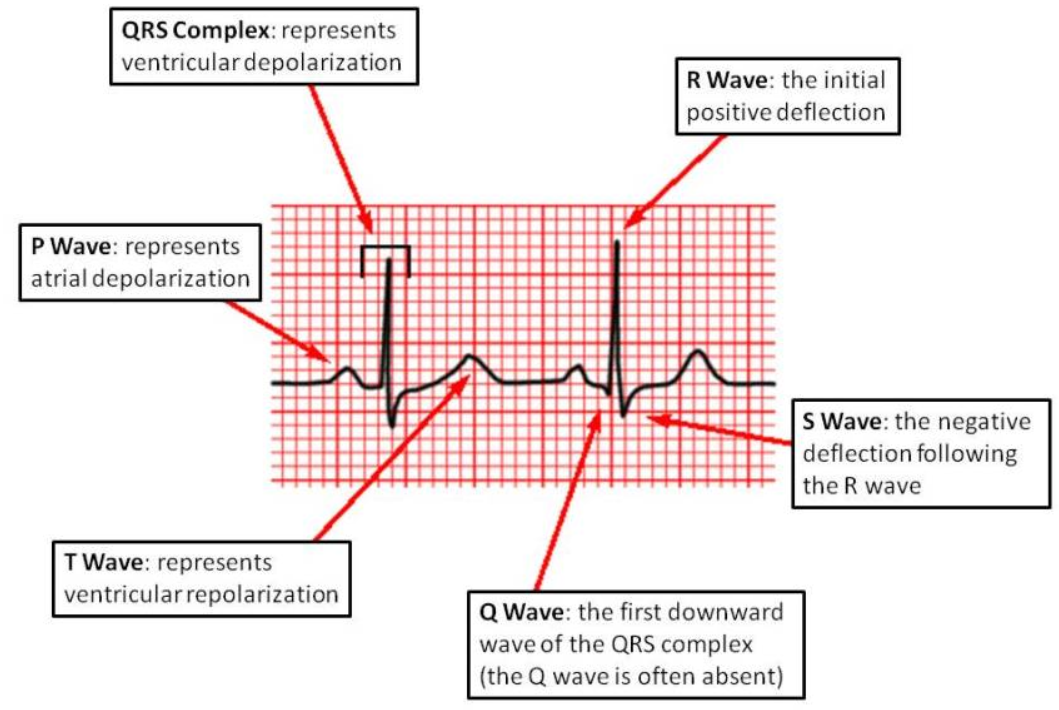
\includegraphics[width=\textwidth]{wave_and_complex}
\caption{}
\end{subfigure}
\caption{(a)12 Lead ECG. (b) Gelombang dan kompleks pada sinyal ECG.}
\captionsetup{font={footnotesize}}
\caption*{sumber : https://meds.queensu.ca/central/assets/modules/ts-ecg/the\_12\_lead\_ecg.html \citep{web3} (diakses tanggal 9 Juni 2018)}
\label{fig:ecg_wave}
\end{figure}

ECG merupakan proses perekaman aktifitas kelistrikan pada jantung menggunakan elektroda yang ditempatkan pada kulit selama periode waktu tertentu. Elektroda ini berfungsi untuk mendeteksi perubahan elektrik kecil pada kulit yang timbul dari pola elektrofisiologis jantung dari depolarisasi dan repolarisasi setiap detak jantung. Hal ini sangat umum dilakukan untuk mendeteksi masalah jantung.
Pada 12-lead ECG konvensional, sepuluh elektroda ditempatkan pada anggota tubuh pasien pada permukaan dada. Besar keseluruhan dari potensi kelistrikan jantung kemudian diukur melalui 12 sudut yang berbeda (Leads) dan dicatat dalam bentuk grafik ---seperti pada Gambar~\ref{fig:ecg_wave}--- selama periode waktu tertentu. Dengan cara ini, besar keseluruhan serta arah depolarisasi kelistrikan jantung dapat didapatkan pada setiap momen sepanjang siklus jantung.


%\begin{figure}[ht]
%\centering
% 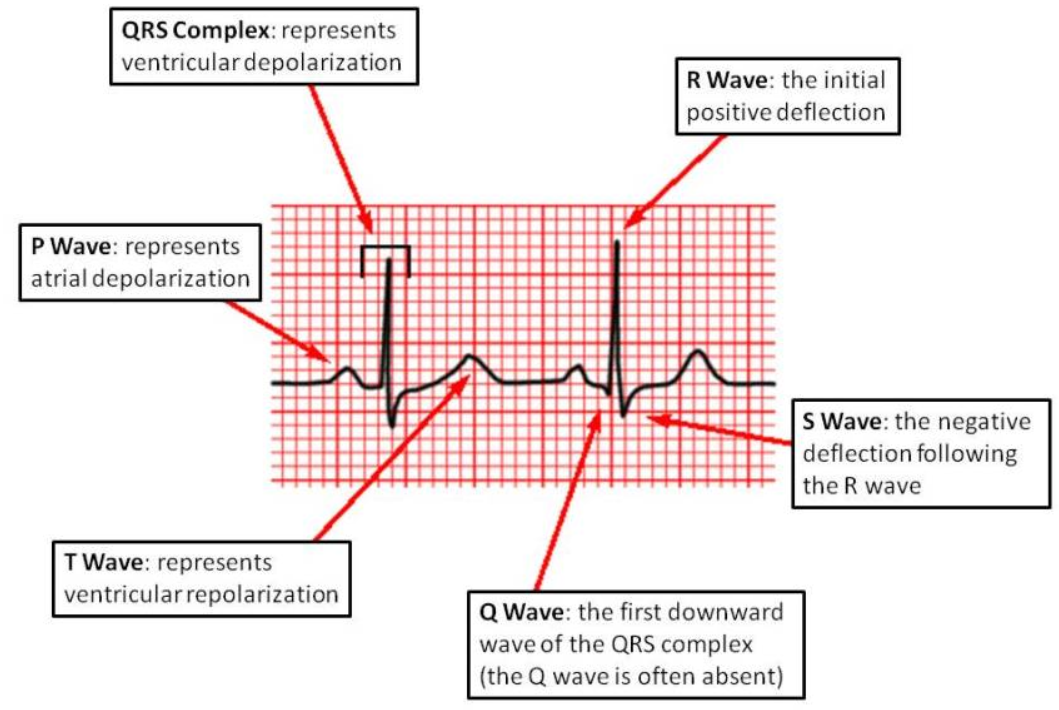
\includegraphics[width=0.6\textwidth]{wave_and_complex}
% \caption{Gelombang dan kompleks pada sinyal ECG.}
%  \captionsetup{font={footnotesize}}  
%  \caption*{sumber : https://meds.queensu.ca/central/assets/modules/ts-ecg/the\_12\_lead\_ecg.html (diakses tanggal 9 Juni 2018)}
% \label{fig:wave_and_complex}   
%\end{figure}

\section{\textit{Photoplethysmography} (PPG)}

\begin{figure}[ht]
%\vspace{0.5em}
	\centering
	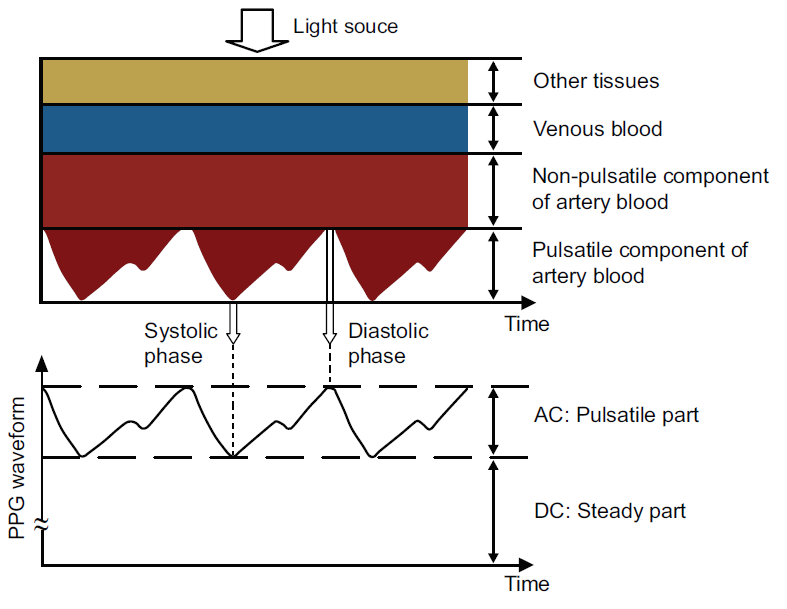
\includegraphics[width=0.8\textwidth]{ppg}
	\caption{Variasi dalam redaman cahaya oleh jaringan tubuh.}
	\captionsetup{font={footnotesize}}  
	\caption*{sumber : Tamura et al. (2014). "Wearable Photoplethysmographic Sensors—Past and Present". Electronics, halaman 2.}
	\label{fig:ppg}   
\end{figure}

Photoplethysmography (PPG) adalah teknik non-invasif untuk mengukur perubahan volume darah mikrovaskular yang terjadi pada wilayah jaringan (\textit{tissue bed}) di bawah lapisan kulit ---yang disebabkan oleh sifat pulsatil dari sistem sirkulasi darah dikarenakan aktifitas jantung berdetak--- dengan menempatkan iluminasi kecil dan probe deteksi pada permukaan kulit [\citet{Allen2007,Kamal1989}]. Karena merupakan teknik optis, PPG membutuhkan sumber cahaya dan fotodetektor untuk berfungsi. Sumber cahaya berfungsi untuk menerangi jaringan tubuh dan fotodetektor untuk merasakan variasi  kecil dalam intensitas cahaya yang dipantulkan atau ditransmisikan berkaitan dengan perubahan perfusi dalam volume tertentu [Ugnell dan Öberg \citep{ugnell1995}]. Prinsip dasar PPG bergantung pada sensitivitas perubahan panjang gelombang optis pada jaringan darah dan jaringan tubuh lainnya. Gambar~\ref{fig:ppg} menunjukkan sistem PPG menghasilkan bentuk gelombang yang dapat mewakili perubahan volume darah yang disebabkan oleh detakan jantung dengan mengukur reflektansi atau transmisi sumber cahaya pada kulit. Metode ini telah terbukti memiliki banyak kegunaan medis dalam pengukuran fitur kardiovaskular seperti denyut jantung, volume darah, saturasi oksigen dan bahkan tingkat respirasi [\citet{Allen2007,Charlton2016}].

\begin{figure}[ht]
%\vspace{0.5em}
\centering
 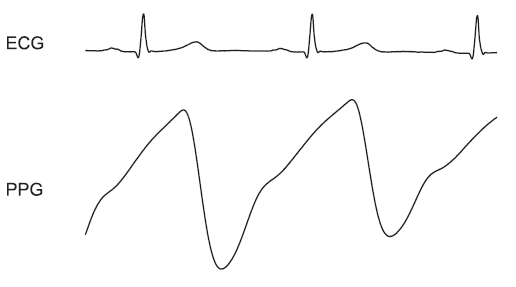
\includegraphics[width=0.6\textwidth]{ecg_and_ppg}
 \caption{Komponen pulsatil (AC) dari sinyal PPG dan sesuai dengan ECG.}
  \captionsetup{font={footnotesize}}  
  \caption*{sumber : Allen, J. (2007). "Photoplethysmography and its application in clinical physiological measurement". Physiol. Meas., halaman 3.}
 \label{fig:ecg_and_ppg}   
\end{figure}

Komponen pulsatil dari gelombang PPG sering disebut komponen 'AC' dan biasanya memiliki frekuensi fundamentalnya sendiri ---biasanya sekitar 1 Hz--- tergantung pada sinyal denyut jantung seperti pada Gambar~\ref{fig:ecg_and_ppg}. Komponen AC ditumpangkan ke komponen kuasi-DC besar yang berhubungan dengan jaringan dan volume darah rata-rata. Komponen DC ini mengalami perubahan secara perlahan karena pengaruh respirasi, aktivitas vasomotorik dan gelombang vasokonstriktor, gelombang Traube Hering Mayer (THM) dan juga termoregulasi [\citet{Allen2007}].



\subsection{Wearable \textit{Photoplethysmography} (PPG)}
Metode Wearable PPG telah banyak dikembangkan dan diaplikasikan secara luas serta diperjualbelikan. Contohnya, pada awal tahun 1990an, \textit{pulse oximetry} digunakan menjadi standar internasional yang dimandatkan untuk monitoring detak jantung selama anestesi [\citet{tremper1989}]. 

\begin{figure}[ht]
	%\vspace{0.5em}
	\centering
	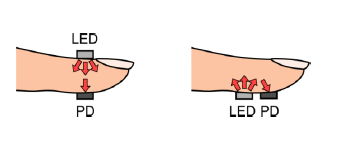
\includegraphics[width=0.4\textwidth]{finger}
	\caption{Penempatan LED dan PD untuk mode transmisi dan reflektansi PPG}
	\captionsetup{font={footnotesize}}  
	\caption*{sumber : Tamura et al. (2014). "Wearable Photoplethysmographic Sensors—Past and Present". Electronics, halaman 4.}
	\label{fig:finger}   
\end{figure}

Menurut \citet{Tamura2014}, Wearable PPG memiliki dua mode ---transmisi dan reflektansi--- seperti yang ditunjukkan pada Gambar~\ref{fig:finger}. Dalam mode transmisi, cahaya yang ditransmisikan melalui medium dideteksi oleh \textit{Photodetector} (PD) yang berlawanan dengan sumber \textit{Light Emitting Diode} (LED), sementara dalam mode reflektansi, PD mendeteksi cahaya yang kembali tersebar atau dipantulkan dari jaringan, tulang dan / atau pembuluh darah. Mode transmisi mampu memperoleh sinyal yang relatif bagus, tetapi daerah pengukuran mungkin terbatas. Agar pengukuran efektif, sensor harus ditempatkan pada tubuh di tempat cahaya yang ditransmisikan dapat dengan mudah dideteksi, seperti ujung jari, septum hidung, pipi, lidah, atau daun telinga. Penempatan sensor pada septum hidung, pipi atau lidah hanya efektif di bawah anestesi. Pada Tabel \ref{table:wearable_PPG} disajikan penelitian yang menggunakan wearable PPG.


\begin{table}[ht]
	\vspace{0.8em}
	\caption{Daftar Penelitian Dengan Wearable PPG}
%	\vspace{0.3em}
	\centering
	\label{table:wearable_PPG}
	\resizebox{.9\textwidth}{!}{%
		\begin{tabular}{| c  c  c  c |}
			\hline 
			Referensi & transmisi/reflektansi & Pengukuran & Letak\\
			\hline
			\citet{Mendelson2006} & reflektansi & HR & Pergelangan tangan \& dahi\\
			\hline
			\citet{Renevey2001} & reflektansi & HR & Pergelangan tangan\\
			\hline
			\citet{Rhee2001} & transmisi & HR & jari manis\\
			\hline
			\citet{Yang1998} & transmisi & HR \& SpO2 & jari manis\\
			\hline
		\end{tabular} 
	}
\captionsetup{font={footnotesize}}
\caption*{Sumber: Sun, Y. and Thakor, N. (2016). Photoplethysmography revisited: from contact to noncontact, from point to imaging. IEEE Transactions on Biomedical Engineering, halaman 4.}
\end{table}

Menurut Sun dan Thakor \citep{sun2016}, meskipun aplikasi dari PPG luas, terdapat beberapa hal signifikan yang membatasi kegunaan dan pengembangan metode PPG konvensional diantaranya :

\begin{itemize}
 \item \textbf{Pengukuran titik}. Sensor PPG hanya dapat memantau perubahan dinamis volume darah pada satu tempat / titik per probe.
 \item \textbf{Kontak saat pengukuran}. Untuk pengukuran yang akurat, sensor PPG konvensional harus melekat kuat pada kulit, yang membatasi kepraktisan dalam situasi seperti diagnosa luka (luka bakar / ulkus / trauma) dan evaluasi penyembuhan kulit atau ketika gerakan bebas diperlukan.
 \item \textbf{Gangguan \textit{motion artifact}}. PPG rentan terhadap kerusakan sinyal yang diinduksi oleh gerakan. Hal itu telah dibuktikan secara klinis bahwa artefak gerak (\textit{motion artifact}) dapat menyebabkan kesalahan dalam respons pulsa oximeter.
 \end{itemize}

%\subsection{PPG Berbasis Kamera}

\subsection{Non-Wearable \textit{Photoplethysmography} (PPG)}
Pengenalan kamera digital untuk sistem pemantauan dan diagnosis pencitraan klinis, keinginan untuk mengurangi pembatasan fisik, dan kemungkinan wawasan baru yang mungkin berasal dari pencitraan perfusi dan pemetaan mendasari pengembangan teknologi PPG konvensional menjadi \textit{vision-based PPG} (PPG berbasis kamera). \textit{Image Photoplethysmography} (iPPG) atau PPG berbasis kamera adalah metode non-kontak yang dapat mendeteksi gelombang denyut jantung yang dihasilkan melalui pengukuran perfusi darah perifer [Sun dan Thakor \citep{sun2016}]. 

\begin{figure}[ht]
%\vspace{0.5em}
\centering
 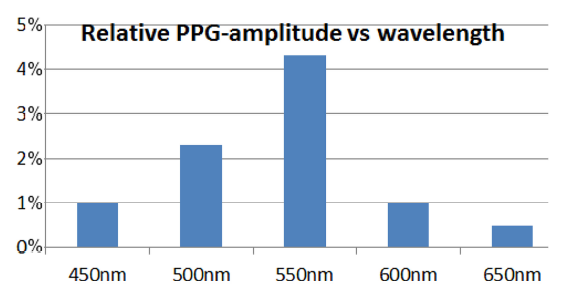
\includegraphics[width=0.8\textwidth]{wavelength}
 \caption{Amplitudo relatif PPG terhadap panjang gelombang PPG berdasarkan penelitian \citet{Crowe1992}}
  \captionsetup{font={footnotesize}}  
  \caption*{sumber : G. de Haan dan V. Jeanne. (2013). "Robust Pulse Rate From Chrominance-Based rPPG," in IEEE Transactions on Biomedical Engineering, halaman 1.}
 \label{fig:wavelength}   
\end{figure}

Pada dasarnya teknik PPG berbasis kamera ini memiliki keuntungan dari fakta bahwa variasi dari penyerapan optis pada kulit manusia bergantung pada panjang gelombang yang digunakan, seperti yang ditunjukkan pada Gambar~\ref{fig:wavelength}. Perubahan gerakan kulit relatif terhadap sensor, di sisi lain, sebagian besar mempengaruhi intensitas cahaya yang dipantulkan atau ditransmisikan oleh kulit tanpa memperhatikan panjang gelombang [de Haan dan Jeanne \citep{deHaan2013}]. \citet{Verkruysse2008} menemukan bahwa sinyal PPG memiliki kekuatan relatif yang berbeda dalam 3 kanal warna (RGB) dari video pada kamera yang ditujukan ke kulit manusia. Beberapa penelitian sebelumnya menggunakan \textit{non-wearable sensor} PPG disajikan pada Tabel \ref{table:vision_PPG}.

%Beberapa penelitian sebelumnya menggunakan \textit{non-wearable sensor} PPG contohnya kamera [de Haan dan Jeanne \citep{deHaan2013}, \citet{Estepp2014,lazaro2014,Mirmo2016,nam2014,Poh2010,Poh2011,Wu2000}] menggunakan metode yang beragam untuk mengolah sinyal PPG yang didapat.

\begin{table}[ht]
%	\vspace{0.8em}
	\caption{Daftar Penelitian \textit{Non-Wearable Vision Based} PPG}
%	\vspace{0.3em}
	\centering
	\label{table:vision_PPG}
	\resizebox{\textwidth}{!}{%
		\begin{tabular}{|l c  c  c  c l|}
			\hline 
			Referensi & Kamera && Pengukuran && Sumber cahaya\\
			\hline
			de Haan dan Jeanne \citep{deHaan2013} & CCD && HR && Lampu studio\\
			\hline
			\citet{Estepp2014}* & CCD && HR && Bola lampu\\
			\hline
			\citet{kong2013} & CCD && HR, BR, \& SpO2 && Cahaya sekitar\\
			\hline
			\citet{Poh2010,Poh2011} & Webcam && HR, BR, \& HRV && Cahaya sekitar\\
			\hline
			\citet{RubinsteinPhDThesis2014} & DC && HR && Cahaya sekitar\\
			\hline
			\citet{Scully2012} & Ponsel && HR, BR, \& SpO2 && LED putih\\
			\hline
			\citet{Verkruysse2008} & DC && HR, BR, \& Perfusi && Cahaya sekitar\\
			\hline
		\end{tabular} 
	}
\vspace{0ex}
\raggedright 
Catatan: CCD = \textit{Charge Coupled Device}; DC = \textit{Digital Camera}; * = Berjalan dalam\newline \hspace*{15mm}mode kontak tanpa penekanan tambahan.
\captionsetup{font={footnotesize}}
\caption*{Sumber: Sun, Y. and Thakor, N. (2016). Photoplethysmography revisited: from contact to noncontact, from point to imaging. IEEE Transactions on Biomedical Engineering, halaman 6.}
\end{table}

%\section{Metode Pengolahan \textit{non-Wearable Sensor} PPG}
\section{\textit{Independent Component Analysis} (ICA)}
Salah satu teknik untuk menghilangkan gangguan (\textit{noise}) dari sinyal fisiologis adalah dengan menggunakan \textit{Blind Source Separation} (BSS). BSS mengacu pada pemulihan sinyal yang tidak teramati atau sumber dari gabungan sinyal yang tidak diketahui sebelumnya bagaimana proses terbentuknya. Biasanya, hasil pengamatan diperoleh dari output satu set sensor, di mana setiap sensor menerima kombinasi sinyal sumber yang berbeda. Ada beberapa metode BSS, salah satunya adalah \textit{Independent Component Analysis} (ICA). ICA adalah teknik untuk mengungkap sinyal sumber independen dari serangkaian pengamatan yang terdiri dari campuran linier dari sumber yang mendasarinya. Dalam penelitian \citet{Poh2010,Poh2011}, sinyal sumber dasar adalah gelombang denyut jantung yang menyebar ke seluruh tubuh. Perubahan volumetrik pembuluh darah di area wajah selama siklus kerja jantung memodifikasi panjang dari garis edar cahaya sekitar yang kemudian mengakibatkan perubahan jumlah cahaya yang dipantulkan yang menunjukkan waktu aktifitas kardiovaskular. Dengan merekam video di daerah wajah menggunakan webcam, sensor warna RGB menangkap campuran sinyal PPG yang dipantulkan bersama dengan sumber lain dari fluktuasi cahaya karena artefak seperti gerak dan perubahan dalam kondisi pencahayaan sekitar. Mengingat bahwa tingkat penyerapan hemoglobin berbeda pada rentang spektral yang terlihat dan dekat-inframerah [\citet{Zijlstra1991}], setiap sensor warna merekam campuran sinyal sumber asli dengan bobot yang sedikit berbeda.

\begin{figure}[ht]
\vspace{0.5em}
\centering
 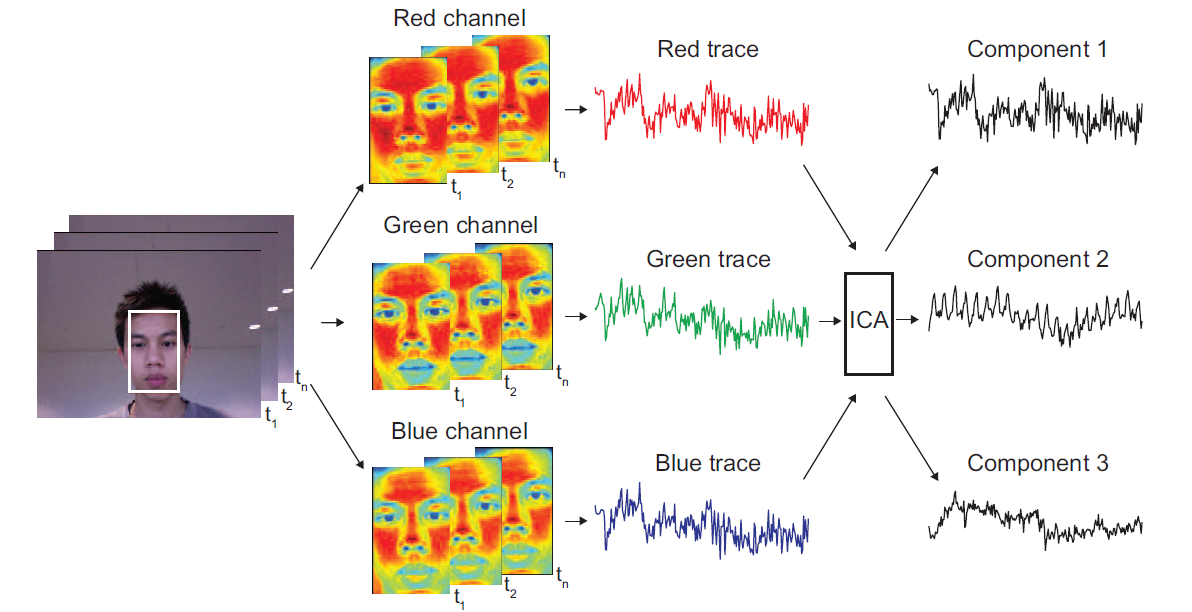
\includegraphics[width=\textwidth]{ICA}
 \caption{Aplikasi Metode ICA untuk memperoleh gelombang PPG}
  \captionsetup{font={footnotesize}}  
  \caption*{sumber : Poh et al, 2010. "Non-contact, automated cardiac pulse measurements using video imaging and blind source separation". Opt. Express, halaman 6.}
 \label{fig:ICA}   
\end{figure}

ICA dapat diterapkan untuk memisahkan data PPG dari artefak gerak, cahaya sekitar (\textit{ambient light}) dan gangguan lain dalam kondisi lingkungan gerak rendah. Penggunaan ICA menarik karena tidak memerlukan pengetahuan seebelumnya dari sistem. Namun, ICA mengasumsikan bahwa semua pasangan komponen sinyal sumber saling independen. Penting untuk menilai kemandirian statistik dari komponen sumber dalam data PPG, terutama jika ICA harus diterapkan dalam lingkungan pemantauan rawat jalan, di mana artefak gerakan dapat memiliki efek substansial pada kualitas data yang diterima dari sensor berbasis cahaya [\citet{Tamura2014}].

\section{\textit{Principle Component Analysis} (PCA)}
Pemfilteran adaptif yang dikombinasikan dengan peningkatan desain mekanik dan konfigurasi probe meningkatkan akurasi sinyal PPG yang dihasilkan [\citet{Rhee2001}]. Kekokohan gerakan (\textit{motion robustness}) dapat diperoleh dengan menggunakan sinyal referensi gerakan yang akurat dari (\textit{low-noise}) akselerometer tiga dimensi (3D), bersama dengan penginderaan inframerah (IR) saluran ganda. Pemodelan nonlinier dan keragaman spasial dari sensor dapat digunakan untuk menghapus kontribusi gerakan ---artefak gerak--- dalam sinyal optik dan kontribusi timbal balik pada masing-masing saluran. \textit{Principle Component Analysis} (PCA) ---yang juga merupakan bagian dari metode BSS--- memanfaatkan korelasi spasial dan temporal di antara dan di dalam gangguan (noise) sinyal yang diamati. Konsep dasar dari pengurangan gangguan berbasis PCA adalah untuk mengamati gangguan data dalam ruang dimensi-m (\textit{m-dimensional space}) yang besar dari koordinat yang tertunda. Karena gangguan diasumsikan sebagai sesuatu yang tidak tentu membuatnya dapat berada di setiap aspek secara merata dalam cakupan ruang tertentu. Sebaliknya, dinamika penetapan sistem pokok untuk membatasi lintasan sinyal yang berguna menjadi sub-ruang dimensi yang lebih rendah (p < m). Oleh karena itu, ruang Eigen (\textit{Eigenspace}) dari beragam gangguan yang diamati dipisahkan menjadi gangguan (\textit{noise}) dan subruang sinyal dan gangguan.

%\subsection{Periodic Moving Average Filter (PMAF)}
%Metode rata-rata bergerak (\textit{Moving Average Filter}) umumnya digunakan untuk mengurangi artefak gerak dan bekerja dengan baik dalam jangkauan artefak yang terbatas. Namun, metode ini tidak dapat memperhitungkan perubahan gerak mendadak. Filter PMAF berdasarkan sinyal PPG yang bersifat kuasi-periodik, membagi sinyal PPG ke dalam beberapa periode dan melakukan sampel ulang pada setiap periode. Dengan begitu metode PMAF dapat menghilangkan artefak gerak tanpa menurunkan kualitas sinyal (Lee et al, 2007). Gangguan in-band (\textit{in-band noise}) terjadi ketika spektrum artefak gerak dan sinyal PPG tumpang tindih secara signifikan. Namun, tidak disarankan untuk menggunakan teknik penyaringan frekuensi tetap (\textit{fixed-frequency}) untuk menghilangkan artefak gerak karena gangguan in-band dan spektrum frekuensi yang tumpang tindih dalam sinyal PPG. Sebaliknya, artefak gerak dapat dihilangkan menggunakan bank filter dan filter yang sesuai yang terdiri dari beberapa pita frekuensi (Lee et al, 2004). Dalam hal ini, filter adaptif menunjukkan banyak perbedaan dan kesalahan dikarenakan variasi amplitudo selama konvergensi ketika mengukur PPG secara real-time, sedangkan MAF menunjukkan output yang lebih stabil (Lee et al, 2004).

%\subsection{Fourier Analysis}
%Penggunaan deret Fourier hanya berlaku untuk sinyal yang periodik, oleh karena itu tidak dapat diterapkan secara langsung pada sinyal PPG karena sifatnya yang tidak statis dan kuasi-periodik. Untuk mengatasi masalah tersebut analisa deret Fourier dapat diterapkan dengan basis siklus demi siklus. Dalam hal ini, data yang diperoleh pertama-tama disaring dengan menggunakan filter Savitzky-Golay (SG) untuk menghilangkan gangguan frekuensi tinggi. Setelah gangguan dihilangkan, analisa deret fourier siklus demi siklus (\textit{cycle-by-cycle Fourier series}) dilakukan dan sinyal PPG (IR dan merah) direkonstruksi secara siklus demi siklus. Hasil penelitian (Reddy et al, 2009) telah membuktikan keberhasilan metode yang digunakan. Selain itu, hasil penelitian juga menunjukkan bahwa artefak gerak yang diinduksi oleh gerakan pasien dapat dilemahkan setidaknya 35 dB yang mengakibatkan pengurangan kesalahan pengukuran sinyal PPG dari 37\% menjadi 3\% menggunakan teknik yang diusulkan.

%\subsection{Kalman Filter}
%Pada penelitian (Lee et al, 2010) penggunaan Kalman filter dapat digunakan untuk memperkirakan pengurangan artefak gerak dan telah terbukti memberikan informasi yang akurat dari sinyal PPG yang direkonstruksi. Dengan menggunakan struktur data khusus dalam Kalman filter estimasi sinyal PPG yang sebenarnya dapat diperoleh. Pada studi (Seyeditabaii, S. dan Seyedtabaii, L., 2008) gerakan jari disimulasikan dan digunakan sebagai referensi gangguan. Sinyal PPG yang terkontaminasi oleh gangguan digunakan sebagai sinyal utama dan algoritma yang diusulkan mampu mengekstrak sinyal utama dari gangguan dalam pita frekuensi yang sama, tidak seperti metode filter yang konvensional.

\section{\textit{Eulerian Video Magnification} (EVM)}
\textit{Eulerian Video Magnification} (EVM) merupakan metode komputasional untuk menghitung dan juga menjadi metode untuk menguatkan proses perubahan kecil/halus ke sinyal data video. Metode ini digunakan untuk menampilkan perubahan warna ataupun pergerakan translasional yang sulit atau tidak dapat dilihat dengan kasat mata. EVM menggunakan rangkaian video standar sebagai masukan (\textit{input}) kemudian menerapkan dekomposisi spasial diikuti dengan pemfilteran sementara (\textit{temporal filtering}) terhadap frame. Sinyal yang dihasilkan kemudian akan dimagnifikasi untuk mengungkap informasi yang tersembunyi. Pada penelitian \citet{Wu2012}, metode EVM dapat memvisualisasikan aliran darah saat melewati wajah dan juga mengungkap pergerakan kecil/halus. Pendekatan dasar yang digunakan adalah untuk memperhatikan rangkaian waktu (\textit{time series}) dari nilai suatu warna pada setiap lokasi ---spasial berupa piksel--- dan memperkuat variasi dalam suatu pita frekuensi waktu yang diberikan.


\begin{figure}[ht]
\vspace{0.5em}
\centering
 \includegraphics[width=\textwidth]{EVM}
 \caption{Kerangka Kerja Metode EVM}
  \captionsetup{font={footnotesize}}  
  \caption*{sumber : Wu et al. (2012). "Eulerian Video Magnification for Revealing Subtle Changes in the World". ACM Trans. Graph., halaman 1. }
 \label{fig:EVM}   
\end{figure}

Melalui proses deteksi dan perbesaran variasi warna halus/kecil ---0,5 unit intensitas dalam skala 8 bit--- dari kulit manusia yang disebabkan oleh aliran darah, HR dapat diekstraksi secara baik dari video RGB standar di mana setiap piksel mencatat nilai intensitas antara 0-255. Biasanya, kualitas sinyal pulsa yang diekstraksi dari titik yang berbeda pada wajah maupun bagian tubuh yang lain dapat bervariasi. Hal ini dikarenakan amplitudo sinyal dapat dimodulasi sesuai dengan kepadatan pembuluh darah perifer, serta karena adanya kontras spasial yang tinggi dari tubuh atau wajah yang membuat lebih sulit untuk mengekstrak sinyal. Selain itu juga terdapat kemungkinan adanya kesalahan dalam mendeteksi puncak pada sinyal bandpass yang digunakan.
Perbedaan penting dari metode pengukuran PPG menggunakan kamera sebelumnya [\citet{kong2013,lazaro2014,lewandowska2011,Mirmo2016,Poh2010,Poh2011,Sun2012,Verkruysse2008}] menggunakan nilai rata-rata piksel di seluruh wilayah wajah, sementara metode EVM hanya dengan mengamati daerah pulsatil di wajah yang akan digunakan untuk mengestimasi nilai HR. 

\subsection{\textit{Space-time Video Processing}}
Meninjau wilayah lokal yang tetap dalam sebuah video. Perubahan warna di wilayah lokal dapat dikaitkan dengan salah satu dari dua sebab yang memungkinkan: (a) objek statis di dalam kawasan telah berubah warna, dan (b) objek di wilayah tersebut telah berpindah, dalam kejadian di mana wilayah tersebut sekarang mungkin memuat bagian yang berbeda dari objek yang ada sebelumnya, atau objek yang berbeda sama sekali. Mengamplifikasi perubahan warna tersebut secara lokal dan mengembalikannya ke dalam video akan membuatnya lebih terlihat oleh mata manusia.

\citet{RubinsteinPhDThesis2014} menggabungkan pemrosesan spasial dan temporal untuk mempertegas perubahan temporal yang halus dalam suatu video. Proses tersebut diilustrasikan pada Gambar~\ref{fig:EVM}. Hal pertama yang dilakukan adalah menguraikan urutan video ke dalam pita frekuensi spasial yang berbeda. Pita-pita frekuensi tersebut mungkin dimagnifikasi secara berbeda karena (a) mereka mungkin menunjukkan rasio signal-to-noise yang berbeda, atau (b) mereka mungkin mengandung frekuensi spasial yang penaksiran linearnya tidak berlaku digunakan dalam \textit{Eulerian Motion Magnification} (sub-bab \ref{ssec:EMM}). Besaran amplifikasi dikurangi untuk pita-pita frekuensi tertentu untuk mengurangi atau menekan artefak gerak. Proses tersebut umumnya dilakukan dengan menggunakan perhitungan piramida Laplacian penuh oleh Burt dan Adelson \citep{burt1987}.

Pemrosesan temporal pada setiap pita spasial dilakukan dengan mempertimbangkan rangkaian waktu yang sesuai dengan nilai piksel dalam pita frekuensi dan menerapkan bandpass filter untuk mengekstrak pita frekuensi yang dibutuhkan. Sebagai contoh, rentan frekuensi dapat dipilih dalam 0.4-4 Hz yang mengimplementasikan 24-240 denyut per menit. Gambar~\ref{fig:compare} menunjukkan rentan nilai frekuensi dan piksel-piksel yang diwakili. Rentan frekuensi tersebut dapat diatur dan dapat dipersempit di sekitar nilai data denyut nadi ketika telah berhasil diekstrak. Pemrosesan temporal seragam untuk semua tingkat spasial, dan untuk semua piksel dalam setiap level.


\subsection{\textit{Eulerian Motion Magnification}} \label{ssec:EMM}
Menurut \citet{RubinsteinPhDThesis2014}, terdapat banyak piksel di daerah wajah terutama yang berada dalam wilayah kontak spasial tinggi tidak memberikan informasi aktifitas jantung yang dapat diandalkan, seperti yang terlihat pada Gambar~\ref{fig:compare}. Dengan begitu, rata-rata yang didapatkan atas daerah deteksi seperti yang dilakukan dalam penelitian sebelumnya [\citet{Poh2010,Poh2011}] dapat mengurangi rasio \textit{signal-to-noise} (SNR) dan keakuratan perkiraan HR.


\begin{figure}[ht]
\vspace{0.5em}
\centering
 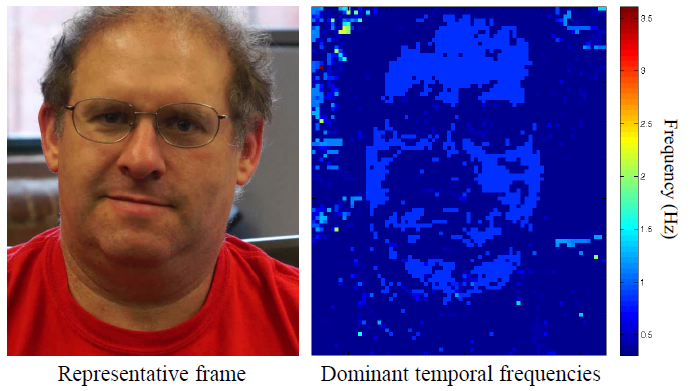
\includegraphics[width=0.8\textwidth]{Compare}
 \caption{Visualisasi frekuensi temporal yang dominan}
  \captionsetup{font={footnotesize}}  
  \caption*{sumber : M. Rubinstein. (2014). "Analysis and visualization of temporal variations in video". PhD thesis, halaman 97.}
 \label{fig:compare}   
\end{figure}

Untuk menjelaskan hubungan antara pemrosesan sementara dan pembesaran gerakan, \citet{Wu2012} mempertimbangkan kasus sederhana dari sinyal 1D yang menjalani gerakan translasi. Analisis ini merupakan generalisasi langsung ke gerak translasi lokal dalam 2D.
Menggunakan \(I(x; t)\) untuk menunjukkan intensitas gambar pada posisi \(x\) dan waktu \(t\). Karena gambar mengalami gerakan translasi, intensitas pengamatan dapat diekspresikan dengan fungsi perpindahan \(\delta (t)\), sehingga \({I(x; t)  =  f(x  +  (t))}\) dan \({I(x; 0)  =  f(x)}\). Tujuan dari pembesaran gerakan adalah untuk mensintesis sinyal
%\begin{spacing}{0.9}
\begin{equation}\label{eq:2.1}
\begin{aligned}
\hat {I}(x;t) = f(x + (1 + \alpha )\delta (t))
\end{aligned}
\end{equation}
Untuk faktor amplifikasi disimbolkan sebagai \(\alpha \).\newline
%\end{spacing}

Dengan asumsi bahwa gambar dapat didekati dengan menggunakan orde pertama deret Taylor sehingga gambar ditulis dalam waktu \(t\), \(f(x + (1 + \alpha )\delta (t))\) dalam ekspansi orde pertama Taylor terhadap \(x\), sebagai
%\begin{spacing}{0.9}
\begin{equation} \label{eq:2.2}
\begin{aligned}
I(x; t) \approx f(x) + \delta {\rm{(}}t{\rm{)}}\frac{{\partial f(x)}}{{\partial x}}.
\end{aligned}
\end{equation}
%\\
%\end{spacing}

Misalkan \(B(x; t)\) merupakan hasil penerapan filter bandpass ---dengan jangkauan frekuensi yang luas--- sementara pada \(I(x; t)\) di setiap posisi \(x\) (kecuali pada \(f(x)\) dalam Persamaan \ref{eq:2.2}). Untuk saat ini, asumsikan sinyal gerak \(\delta (t)\) berada di dalam passband dari filter bandpass sementara (\textit{temporal bandpass filter}) ---asumsi akan dilonggarkan nanti---, sehingga
%\begin{spacing}{0.9}
\begin{equation} \label{eq:2.3}
\begin{aligned}
B(x; t)  = \delta {(t)}\frac{{\partial f(x)}}{{\partial x}}.
\end{aligned}
\end{equation}
%\\
%\end{spacing}


Dalam prosesnya, sinyal handpass kemudian diamplifikasi dengan \(\alpha \) dan menambahkannya kembali ke \(I(x; t)\), menghasilkan sinyal yang telah diproses
%\begin{spacing}{0.9}
\begin{equation} \label{eq:2.4}
\begin{aligned}
{\tilde I(x; t)  =  I(x; t)  +  }\alpha {B(x; t)}.
\end{aligned}
\end{equation}
%\\
%\end{spacing}


Dengan menggabungkan Persamaan \ref{eq:2.2}, \ref{eq:2.3}, dan \ref{eq:2.4}, sehingga didapatkan 
%\begin{spacing}{0.9}
\begin{equation} \label{eq:2.5}
\begin{aligned}
\tilde I(x; t) \approx {f(x)  +  (1 + }\alpha)\delta {(t)}\frac{{\partial f(x)}}{{\partial x}}.
\end{aligned}
\end{equation}
%\\
%\end{spacing}

Dengan mengasumsikan ekspansi orde pertama Taylor berlaku untuk mengamplifikasi gangguan yang lebih besar \((1 +\alpha)\delta{(t)}\), amplifikasi dari sinyal bandpassed sementara dengan magnifikasi gerakan dapat direlasikan. Luaran yang diproses adalah
%\begin{spacing}{0.9}
\begin{equation} \label{eq:2.6}
\begin{aligned}
\tilde I(x; t) \approx f(x  +  (1  + \alpha )\delta (t)).
\end{aligned}
\end{equation}
Ini menunjukkan bahwa pengolahan perbesaran gerakan ---perpindahan spasial  \(\delta (t)\) dari citra lokal \(f(x)\) pada waktu \(t\)--- telah dimagnifikasi dengan magnitudo \((1+\alpha)\).\\
%\end{spacing}


Proses ini diilustrasikan untuk satu gelombang sinusoid pada Gambar~\ref{fig:Sinus}. Pada gelombang kosinus frekuensi rendah dan perpindahan yang relatif kecil \(\delta (t)\), ekspansi deret Taylor orde pertama berfungsi sebagai pendekatan yang baik untuk sinyal yang ditranslasi pada waktu \(t+1\). Ketika menguatkan sinyal sementara dengan \(\alpha\) dan menambahkannya kembali ke \(I(x; t)\), diperkirakan gelombang tersebut ditranslasi dengan \((1  + \alpha )\delta\).

\begin{figure}[ht]
	\vspace{0.5em}
	\centering
	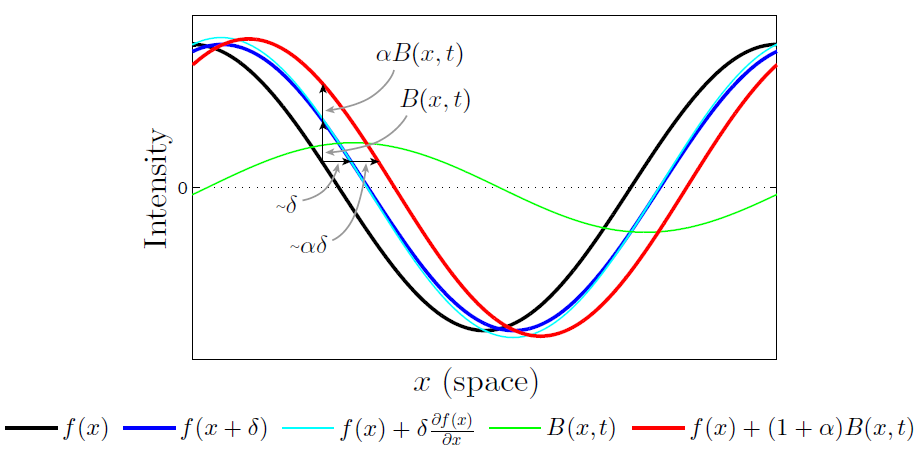
\includegraphics[width=\textwidth]{Sinus}
	\caption[Pemfilteran temporal untuk memperkirakan translasi spasial]{Pemfilteran temporal untuk memperkirakan translasi spasial. Hasil pemfilteran ditunjukkan dalam sinyal 1D, akan tetapi hal tersebut berlaku juga untuk sinyal 2D. Sinyal input ditampilkan pada dua waktu instan: \(I(x; t) = f(x)\) pada waktu \(t\) dan \(I(x; t+1) = f(x + \delta)\) \(t+1\). Urutan pertama ekspansi deret Taylor dari \(I(x; t+1)\) terhadap \(x\) mendekati sinyal yang ditranslasi dengan baik. Bandpass sementara diamplifikasi dan ditambahkan ke sinyal asli untuk menghasilkan translasi yang lebih besar. Dalam contoh ini \(\alpha=1\) memperbesar gerakan sebesar 100\%, dan filter temporal merupakan filter beda hingga (\textit{finite difference}) mengurangkan dua kurva.}
	\captionsetup{font={footnotesize}}  
	\caption*{sumber : Wu et al. (2012). "Eulerian Video Magnification for Revealing Subtle Changes in the World". ACM Trans. Graph., halaman 3.}
	\label{fig:Sinus}   
\end{figure}

Untuk lebih lengkap, kembali dalam kasus yang lebih umum di mana \(\delta (t)\) tidak sepenuhnya berada di dalam passband dari filter temporal. Dalam hal ini \({\delta _k}(t)\) diindeks oleh k, mewakili komponen spektral temporal yang berbeda \(\delta (t)\). Setiap \({\delta _k}(t)\) akan dilemahkan oleh filter temporal berdasarkan faktor \({\gamma _k}\). Hal ini menghasilkan sinyal bandpass,
%\begin{spacing}{0.9}
\begin{equation} \label{eq:2.7}
\begin{aligned}
B(x; t) = \sum\limits_k^{} {{\gamma _k}{\delta _k}(t)\frac{{\partial f(x)}}{{\partial x}}}
\end{aligned}
\end{equation}
%\\
%\end{spacing}
%
(bandingkan dengan Persamaan \ref{eq:2.3}). Lantaran perkalian dalam Persamaan \ref{eq:2.4}, frekuensi temporal yang bergantung redaman dapat diartikan sebagai faktor pembesaran gerak yang bergantung pada frekuensi \({\alpha _k} = {\gamma _k}\alpha\), menghasilkan luaran magnifikasi gerak,
%\begin{spacing}{0.9}
\begin{equation} \label{eq:2.8}
\begin{aligned}
\tilde I(x;t) \approx f(x + \sum\limits_k {(1 + {\alpha _k})} {\delta _k}(t))
\end{aligned}
\end{equation}
%\\
%\end{spacing}

Hasilnya adalah seperti yang diharapkan untuk analisis linear: modulasi komponen spektral dari sinyal gerak menjadi faktor modulasi dalam faktor amplifikasi gerak \(\alpha _k\), untuk setiap sub-band sementara \(\gamma _k\), dari sinyal gerakan.
%!TEX root = ../thesis.tex
%*******************************************************************************
%****************************** Third Chapter **********************************
%*******************************************************************************
\chapter{PERANCANGAN SISTEM}

% **************************** Define Graphics Path **************************
\ifpdf
    \graphicspath{{Chapter3/Figs/Raster/}{Chapter3/Figs/PDF/}{Chapter3/Figs/}}
\else
    \graphicspath{{Chapter3/Figs/Vector/}{Chapter3/Figs/}}
\fi

Pada bab ini akan dibahas lebih dalam mengenai perancangan tugas akhir yang akan dikerjakan. Gambar~\ref{fig:FlowChart} merupakan diagram alir tahapan pengerjaan proyek akhir yang direncanakan. 

\begin{figure}[ht]
 %\vspace{0.5em}
 \centering
 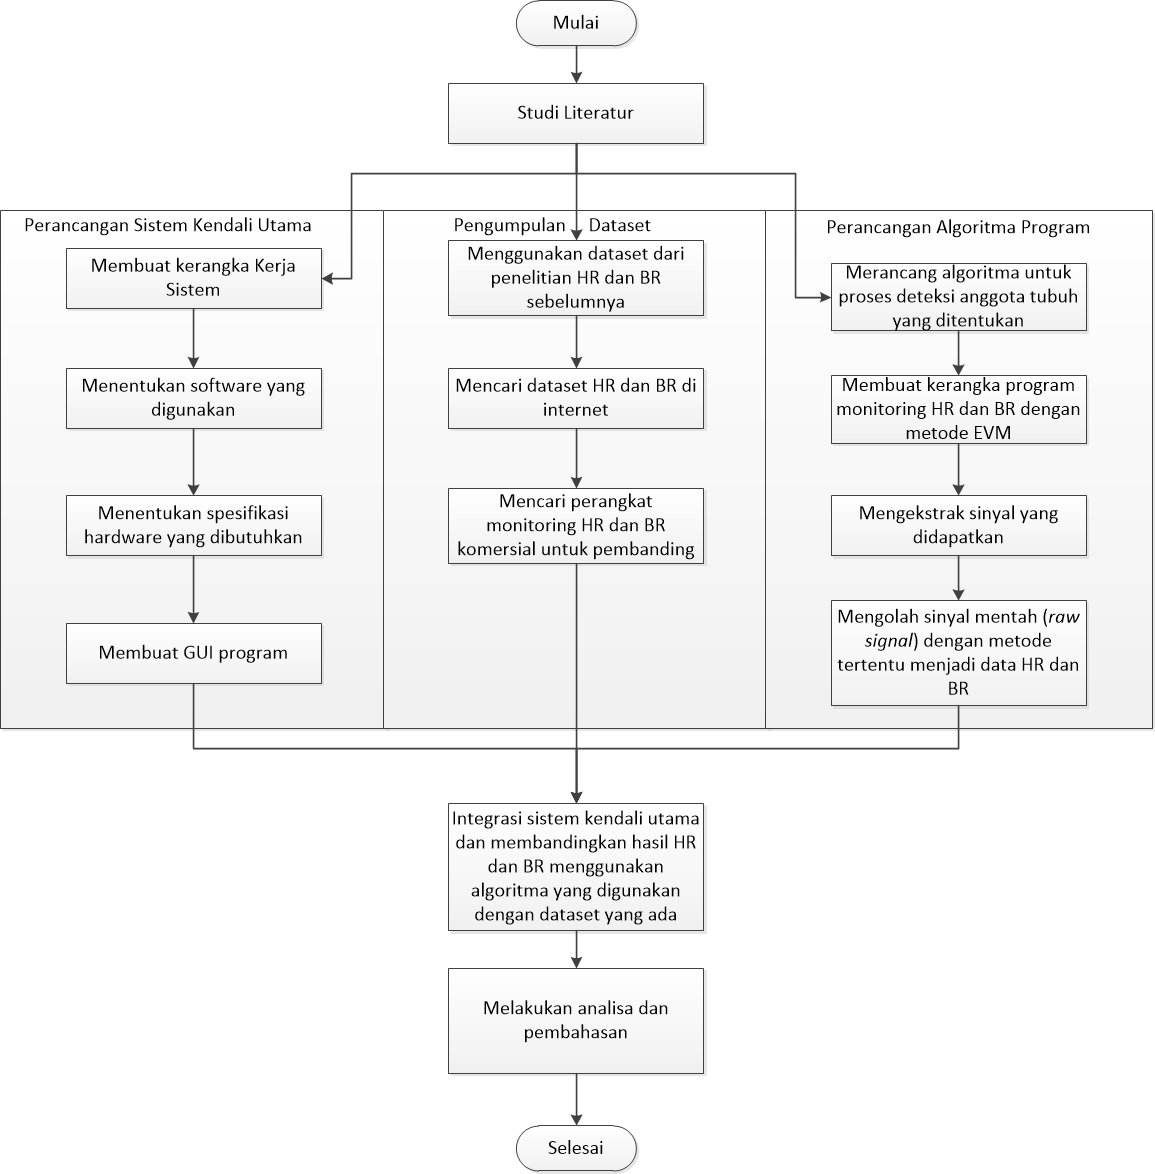
\includegraphics[width=\textwidth]{FlowChart}
 \caption{Diagram Alir Pengerjaan Proyek Akhir}
 \label{fig:FlowChart}   
\end{figure}

\section{Perancangan Sistem Kerja}
Pada bagian ini akan dibahas tentang perancangan sistem yang akan digunakan pada proyek akhir ini. Secara garis besar, proyek akhir ini terdiri atas tiga bagian yaitu mekanisme pendeteksian objek, proses amplifikasi dan ekstraksi sinyal,  dan implementasi pada perangkat sistem benam.


\begin{figure}[ht]
 \vspace{0.5em}
 \centering
 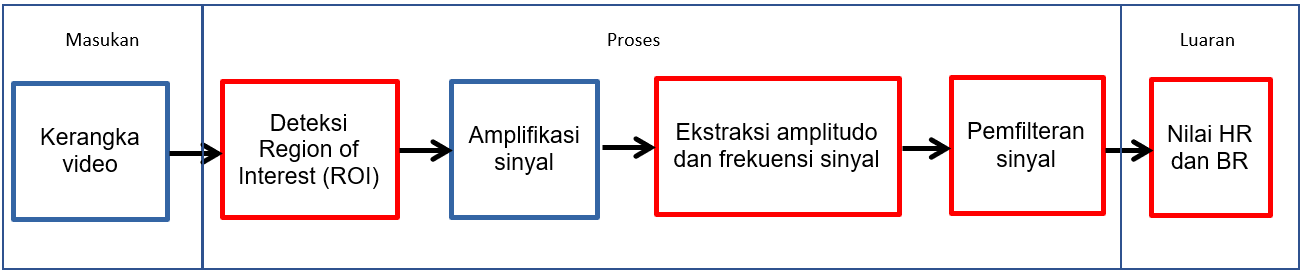
\includegraphics[width=\textwidth]{diagramblok}
 \caption{Perancangan Sistem Kerja}
 \label{fig:diagramblok}   
\end{figure}

Seperti terlihat pada Gambar~\ref{fig:diagramblok}, fokus dari proyek akhir ini ditandai oleh warna merah. Masukan dari proyek akhir ini berupa kerangka video ---diambil menggunakan kamera--- pada bagian tubuh tertentu yang diketahui dapat menunjukkan informasi adanya aktifitas pernapasan maupun sirkulasi darah seperti pada pergelangan tangan, leher, perut dan kepala. Setelah itu kerangka video yang didapat akan diolah pada sistem kendali utama melalui proses pendeteksian area yang menunjukkan adanya perubahan informasi dalam piksel yang berkaitan dengan adanya aktifitas pernapasan maupun sirkulasi darah. Informasi yang berupa sinyal tersebut kemudian akan diamplifikasi dengan menggunakan kerangka dari metode \textit{Eulerian Video Magnification} (EVM) dan akan dilakukan proses ekstraksi ampitudo dan frekuensi dari sinyal tersebut sebagai data mentah untuk diolah lebih lanjut. Proses pengolahan dan pemfilteran sinyal yang merupakan pekerjaan utama dari proyek akhir ini akan dilakukan dengan menggunakan metode yang akan dirancang pada saat pengerjaan proyek akhir. Melalui proses pengolahan data tersebut akan dihasilkan luaran berupa nilai konkret dari HR dan BR yang terdeteksi.

\section{Spesifikasi Hardware}
\subsection{Kamera}
Peran kamera dalam proyek akhir ini sangatlah penting. Kamera merupakan salah satu faktor penting dalam proyek akhir ini karena masukan utama yang digunakan adalah data visual. Pemilihan model kamera yang akan digunakan dapat mempengaruhi kualitas dari video yang ditangkap dan tidak menutup kemungkinan bahwa hal tersebut bisa berdampak pada luaran yang dihasilkan. Semakin besar kapasitas piksel yang dimiliki, maka semakin banyak informasi yang dihasilkan. Namun, hal tersebut dapat mengakibatkan proses pengolahan data menjadi lebih lama. Oleh karena itu, pemilihan model kamera perlu diperhatikan. Pada Tabel \ref{table:spek_cam} disajikan model kamera yang dapat dijadikan opsi dalam pengerjaan proyek akhir ini.

\begin{table}[ht]
\vspace{0.8em}
\caption[Kamera untuk Proses Monitoring HR dan BR]{Contoh Kamera untuk Proses Monitoring HR dan BR}
%\vspace{0.3em}
\centering
\label{table:spek_cam}
\resizebox{.8\textwidth}{!}{%
\begin{tabular}{| c | c |}
\hline 
Model & Spesifikasi \\
\hline
Kinect & Up to 640x480 pixels @30 fps \\
& \textbf{RGB + IR depth-finding}\\
\hline
Netatmo Presence Camera & Up to 1920x1080 pixels \\
& \textbf{RGB + IR}\\
& Deteksi hingga 15 meter\\
& Konektifitas hanya melalui Wifi\\
\hline
Netgear Arlo Q & Up to 1920x1080 pixels HD @30 fps \\
& \textbf{CMOS-RGB + IR}\\
& Deteksi hingga 15 meter\\
& 8x digital zoom\\
\hline
Hikvision Ezviz Mini Plus & Up to 1920x1080 pixels \\
& \textbf{RGB + IR}\\
& Konektifitas hanya melalui Wifi\\
\hline
Logitech 4K Pro Webcam & Up to 4096 x 2160 pixels HD @30 fps \\
& \textbf{RGB + IR}\\
& 5x digital zoom\\
\hline
Logitech C922 Webcam & Up to 1920x1080 pixels HD @30 fps\\
& \textbf{RGB}\\
\hline
Logitech C525 Webcam & Up to 1280 x 720 pixels HD @30 fps\\
& \textbf{RGB}\\
\hline 
\end{tabular} 
}
\end{table}

Kamera kinect memiliki kellebihan dengan adanya teknologi \textit{IR depth-finding} atau yang biasanya dikenal dengan sebutan teknologi RGBd yang dapat memvisualisasikan kedalaman (\textit{depth}) dari suatu obyek. Hal tersebut dapat menjadi suatu kebaruan dalam penelitian mengenai PPG untuk mengetahui pemanfaatan teknologi \textit{IR depth-finding} dalam proses monitoring HR dan BR.

\subsection{ Spesifikasi Perangkat Benam \textit{Embedded Platform}}
Meskipun pengujian algoritma dan sistem menggunakan dilakukan pada \textit{Personal Computer} (PC) atau laptop, namun tujuan dari proyek akhir ini adalah membuat sistem embedded yang digunakan untuk melakukan monitoring HR dan BR yang \textit{non-wearable}. Oleh karena itu, diperlukan perangkat benam yang dapat menjalankan tugas tersebut dengan baik. Hal ini penting mengingat pekerjaan yang dilakukan meliputi pengolahan citra digital serta pengolahan sinyal digital yang memerlukan kecepatan komputasi yang tinggi untuk mendukung keandalan dari sistem. Pengukuran nilai HR dan BR sebisa mungkin dilakukan dalam kondisi \textit{real time} dengan jeda waktu yang singkat mengingat urgensinya. Proses pengolahan citra dan sinyal memerlukan perangkat benam degan CPU dan GPU yang tinggi seperti yang disajikan pada Tabel \ref{table:spek_pc}.

\begin{table}[ht]
\vspace{0.8em}
\caption{Spesifikasi Perangkat Benam untuk Prosas Monitoring HR dan BR}
%\vspace{0.3em}
\centering
\label{table:spek_pc}
\resizebox{\textwidth}{!}{%
\begin{tabular}{| c c |}
\hline 
Model & Spesifikasi \\
\hline
Intel® NUC Kit & Up to 4.20 GHz (4 cores, 8 threads) \\
GPU & \textbf{Up to Radeon™ RX Vega M GH graphics } \\
\hline
Jetson TK1 & NVIDIA "4-Plus-1" 2.32GHz ARM quad-core Cortex-A15 CPU\\
GPU & \textbf{NVIDIA Kepler "GK20a" GPU with 192 SM3.2 CUDA cores (up to 326 GFLOPS)}\\
\hline
Jetson TX1 & Quad ARM® A57/2 MB L2 @1.9 GHz\\
GPU & \textbf{NVIDIA Maxwell ™, 256 CUDA cores}\\
\hline
Jetson TX2 & HMP Dual Denver 2/2 MB L2 @1.4–2.0 GHz + Quad ARM® A57/2 MB L2U @1.2–2.0 GHz \\
GPU & \textbf{NVIDIA Pascal™, 256 CUDA cores}\\
\hline
ODROID-XU4 & Samsung Exynos5422 Cortex™-A15 2Ghz and Cortex™-A7 Octa core CPUs\\
GPU & \textbf{Mali-T628 MP6(OpenGL ES 3.1/2.0/1.1 and OpenCL 1.2 Full profile)}\\
\hline
MintBox 2 & Intel Core i5-3337U dual coreProcessor @1.8GHz (turbo boost up to 2.7GHz)\\
GPU & \textbf{Intel HD Graphics 4000}\\
\hline 
\end{tabular} 
}
\end{table}

Berdasarkan Tabel  \ref{table:spek_pc}, Intel NUC merupakan satu-satunya perangkat yang memiliki kelebihan dalam hal fleksibilitas dikarenakan beberapa komponen dapat dibongkar pasang dan dapat ditingkatkan spesifikasinya sedangkan perangkat lain bersifat tertanam sepenuhnya sehingga memiliki spesifikasi yang tidak dapat diubah.




\section{Perancangan \textit{Graphical User Interface} (GUI)}
Pembuatan \textit{Graphical User Interface} (GUI) bertujan untuk menampilkan proses pengolahan data serta monitoring dan menampilkan data secara \textit{real time} dari kamera yang berfungsi sebagai sensor dalam proses monitoring tingkat HR dan BR pada tubuh. GUI dirancang dengan menggunakan aplikasi matlab yang juga digunakan untuk melakukan proses komputasi dan pengolahan data. Berdasarkan perancangan GUI yang dapat dilihat pada Gambar~\ref{fig:gui}, terdapat dua kotak yang nantinya akan diisi dengan frame video yang akan digunakan untuk menampilkan video masukkan yang dihasilkan dari kamera serta video luaran yang telah diproses. Selain itu, terdapat dua plot diagram yang masing-masing akan digunakan untuk menampilkan data frekuensi dan data amplitudo yang didapatkan selama proses monitoring HR dan BR berlangsung. \textit{Check Box} dapat berisi opsi pengaturan yang dapat digunakan untuk memberikan detil lebih lengkap pada plot diagram yang dibuat. Tombol \textit{Push Button} akan digunakan untuk memulai dan mengakhiri proses monitoring. Pada \textit{Pop-up Menu} dapat digunakan untuk mengubah tampilan yang ada pada GUI.

\begin{figure}[ht]
 \vspace{0.8em}
 \centering
 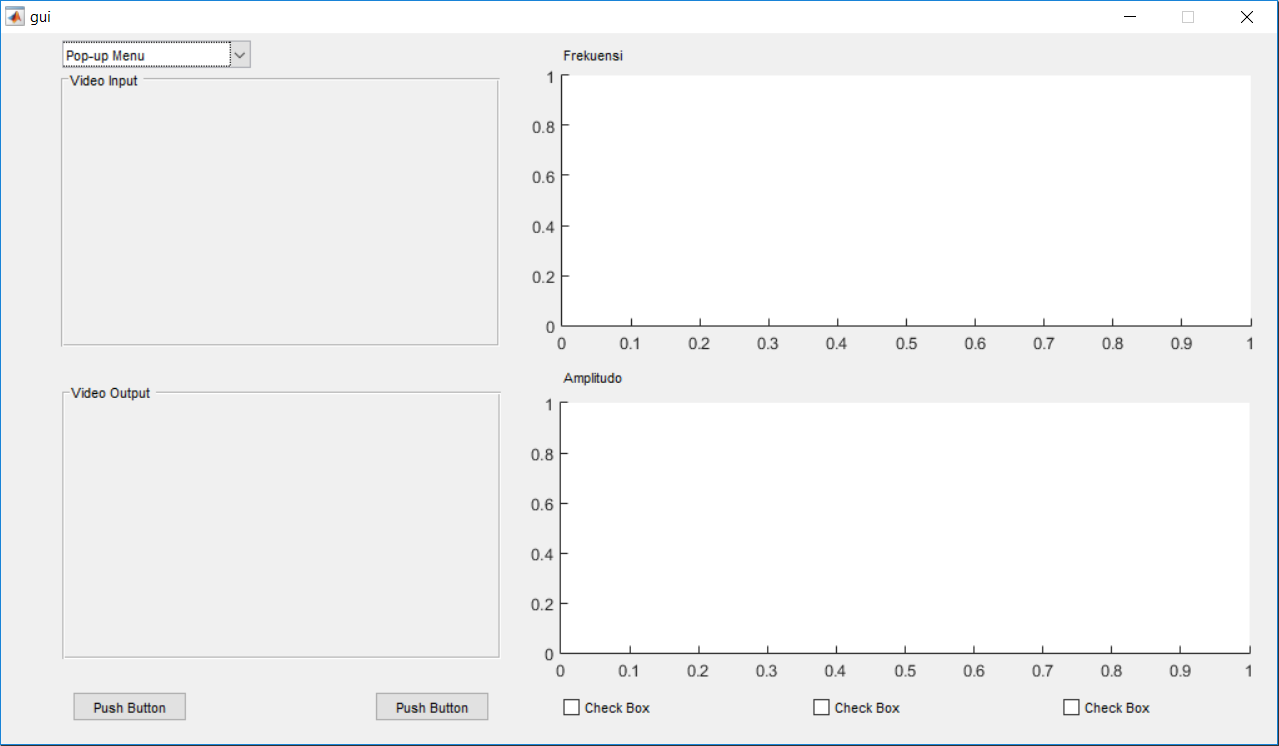
\includegraphics[width=0.8\textwidth]{gui}
 \caption{Rancangan \textit{Graphical User Interface} (GUI)}
 \label{fig:gui}   
\end{figure}

\section{Rencana Validasi Data}
Mengingat bahwa proyek akhir yang akan dikerjakan erat kaitannya dengan bidang kesehatan terlebih menyangkut nyawa seseorang, maka diperlukan proses validasi yang kredibel. Proses validasi data dalam bidang kesahatan paling baik dilakukan dengan cara menjalin kerja sama dengan instansi kesehatan yang berkaitan secara langsung. Namun, dikarenakan proyek akhir ini dibuat untuk penggunaan sehari-hari serta meninjau bahwa prosedur kerja sama dengan instansi kesehatan yang tidak mudah, maka rencana validasi yang realistis dapat dilakukan adalah dengan membandingkan hasil monitoring HR dan BR dengan alat-alat yang memiliki fungsi serupa dan sudah diproduksi dan telah diperjualbelikan secara massal. Pada Tabel \ref{table:alat} disajikan beberapa perangkat \textit{wearable} yang dapat digunakan untuk proses validasi data.

\begin{table}[ht]
\vspace{0.8em}
\caption[Perangkat \textit{Wearable} untuk Pengukuran HR dan BR]{Perangkat \textit{Wearable} komersial untuk Pengukuran HR dan BR}
%\vspace{0.3em}
\centering
\label{table:alat}
\resizebox{.9\textwidth}{!}{%
\begin{tabular}{| c c |}
\hline 
Nama Alat & Keterangan \\
\hline
Pulse Oximeter & Pengukuran HR dan SpO2  \\
 	& Pengukuran pada ujung jari\\
\hline
Fitbit Versa Heart Rate Smart Watch & Pengukuran HR dan kualitas tidur\\
 	& Pengukuran pada pergelangan tangan\\
\hline
Xiaomi Amazfit 2 Smart Watch & Pengukuran HR dan kualitas tidur\\
 	& Pengukuran pada pergelangan tangan\\
\hline
Equivital LifeMonitor & Pengukuran HR dan BR \\
 	& Pengukuran pada wilayah dada\\
\hline
Garmin Strap HRM TRI ANT & Pengukuran HR dan variabilitas HR\\
 	& Pengukuran pada wilayah dada\\
\hline 
\end{tabular} 
}
\end{table}

\section{Perencanaan Jadwal Kerja Penelitian Proyek Akhir}

Pada Tabel \ref{tab:jadwalkerja} di bawah adalah jadwal kerja proyek akhir yang telah disusun dan dibuat berdasarkan metodologi dalam pembuatan sistem monitoring HR dan BR.
\begin{table}[ht]
	\vspace{0.8em}
	\setlength{\arrayrulewidth}{1pt}
	\centering
	\caption{Perencanaan Jadwal Kerja Proyek Akhir}
%	\vspace{0.3em}
	\label{tab:jadwalkerja}
	\resizebox{\textwidth}{!}{%
	\begin{tabular}{|c|l|c|c|c|c|c|c|c|c|c|c|c|c|c|c|}
	\hline
	    & 			& \multicolumn{7}{ c| }{Tahun 2018}	& \multicolumn{7}{ c| }{Tahun 2019}\\\cline{3-16}
	No  &\multicolumn{1}{c|}{Kegiatan}&\multicolumn{7}{ c| }{Bulan}&\multicolumn{7}{ c| }{Bulan}	\\ \cline{3-16}
		& 			&6&7&8&9&10&11&12					&1&2&3&4&5&6&7		\\ \hline
	
	1	& Studi Literatur		&\cellcolor{blue!100}&\cellcolor{blue!100}&\cellcolor{blue!100}&\cellcolor{blue!100}&\cellcolor{blue!100}&\cellcolor{blue!100}&\cellcolor{blue!100}&\cellcolor{blue!100}&\cellcolor{blue!100}&\cellcolor{blue!100}&&&&		\\ \hline
	2	& Koding Program		&&&&\cellcolor{blue!100}&\cellcolor{blue!100}&\cellcolor{blue!100}&\cellcolor{blue!100}&\cellcolor{blue!100}&\cellcolor{blue!100}&\cellcolor{blue!100}&\cellcolor{blue!100}&\cellcolor{blue!100}&\cellcolor{blue!100}&		\\ \hline
	3	& Perancangan Sistem	&&&\cellcolor{blue!100}&\cellcolor{blue!100}&\cellcolor{blue!100}&\cellcolor{blue!100}&\cellcolor{blue!100}&\cellcolor{blue!100}&\cellcolor{blue!100}&\cellcolor{blue!100}&\cellcolor{blue!100}&\cellcolor{blue!100}&\cellcolor{blue!100}&		\\ \hline
	4	& Perancangan Mekanik	& &&&&&\cellcolor{blue!100}&\cellcolor{blue!100}&\cellcolor{blue!100}&\cellcolor{blue!100}&\cellcolor{blue!100}&&&&		\\ \hline
	5	& Perancangan GUI		& &&&&&&\cellcolor{blue!100}&\cellcolor{blue!100}&\cellcolor{blue!100}&\cellcolor{blue!100}&\cellcolor{blue!100}&&&		\\ \hline
	6	& Pengujian Sistem		& &&&&&&\cellcolor{blue!100}&\cellcolor{blue!100}&\cellcolor{blue!100}&\cellcolor{blue!100}&\cellcolor{blue!100}&\cellcolor{blue!100}&\cellcolor{blue!100}&		\\ \hline
	7	& Penyusunan Laporan Akhir	&\cellcolor{blue!100}&\cellcolor{blue!100}&\cellcolor{blue!100}&\cellcolor{blue!100}&\cellcolor{blue!100}&\cellcolor{blue!100}&\cellcolor{blue!100}&\cellcolor{blue!100}&\cellcolor{blue!100}&\cellcolor{blue!100}&\cellcolor{blue!100}&\cellcolor{blue!100}&\cellcolor{blue!100}&\cellcolor{blue!100}		\\ \hline
	\end{tabular}
}
\end{table}

%------------------------------------Template Tabel-----------------------%
%\begin{table}[ht]
%	\vspace{0.5em}
%	\centering
%	\caption{Perencanaan Jadwal Kerja Proyek Akhir}
%	\label{tab:jadwalkerja}
%	\resizebox{\textwidth}{!}{%
%		\begin{tabular}{|c|l|c|c|c|c|c|c|c|c|c|c|c|c|c|c|}
%			\hline
%			& 			& \multicolumn{7}{ c| }{Tahun 2018}	& \multicolumn{7}{ c| }{Tahun 2019}\\\cline{3-16}
%			No  &\multicolumn{1}{c|}{Kegiatan}&\multicolumn{7}{ c| }{Bulan}&\multicolumn{7}{ c| }{Bulan}	\\ \cline{3-16}
%			& 			&6&7&8&9&10&11&12					&1&2&3&4&5&6&7		\\ \hline
%			
%			1	& Studi Literatur		& &&&&&&				&		&&&&&&		\\ \cline{1-16}
%			2	& Koding Program		& &&&&&&				&		&&&&&&		\\ \cline{1-16}
%			3	& Perancangan Sistem	& &&&&&&				&		&&&&&&		\\ \cline{1-16}
%			4	& Perancangan Mekanik	& &&&&&&				&		&&&&&&		\\ \cline{1-16}
%			5	& Perancangan GUI		& &&&&&&				&		&&&&&&		\\ \cline{1-16}
%			6	& Pengujian Sistem		& &&&&&&				&		&&&&&&		\\ \cline{1-16}
%			7	& Penyusunan Laporan Akhir	& &&&&&&				&		&&&&&&		\\ \cline{1-16}
%		\end{tabular}
%	}
%\end{table}
%%!TEX root = ../thesis.tex
%*******************************************************************************
%****************************** Third Chapter **********************************
%*******************************************************************************
\chapter{Rencana Pengujian dan Analisa Sistem}

% **************************** Define Graphics Path **************************
\ifpdf
    \graphicspath{{Chapter4/Figs/tinggi/}{Chapter4/Figs/idv/}{Chapter4/Figs/}}
\else
    \graphicspath{{Chapter4/Figs/Vector/}{Chapter4/Figs/}}
\fi

Pada bab ini akan disebutkan rencana pengujian dari sistem. Pengujian meliputi dari pengambilan video, proses pengolahan data serta kumpulan data hasil uji coba.

\section{ Pengujian Pengambilan Video}
\section{ Pengujian Penentuan ROI}
\section{ Pengujian Amplifikasi Video dengan EVM}
\section{ Pengujian Ekstraksi Sinyal}
\section{ Pengujian Pemfilteran Sinyal}
\section{ Hasil Pengujian Menggunakan Sistem Embedded}
%%!TEX root = ../thesis.tex
%*******************************************************************************
%****************************** Third Chapter **********************************
%*******************************************************************************
\chapter{PENUTUP}

% **************************** Define Graphics Path **************************
\ifpdf
    \graphicspath{{Chapter5/Figs/Raster/}{Chapter5/Figs/PDF/}{Chapter5/Figs/}}
\else
    \graphicspath{{Chapter5/Figs/Vector/}{Chapter5/Figs/}}
\fi

\section{Kesimpulan}
Dari hasil uji coba pada penelitian ini dapat ditarik beberapa kesimpulan:
\begin{enumerate}
\item Komunikasi wireless antara Xbee Pro dengan Notebook bisa dilakukan dengan menggunakan komunikasi USB – Serial. 
\item Dengan bantuan beberapa software, komunikasi serial secara wireless dapat diakses dengan mudah.
\item Struktur mekanik sangat berperan penting dalam mempermudah sistem kontrol pada robot, struktur yang kokoh dari sebuah robot sangat mempengaruhi tingkat kerumitan saat robot diprogram.
\item Robot iSRo dapat dikendalikan seraca manual dan wireless.
\end{enumerate}

\section{Saran}
Pada serangkaian uji coba dan penelitian yang dilakukan selama ini, robot iSRo dapat dikemudikan dengan menggunakan manual dan wireless. Dengan menggunakan bantuan beberapa software komunikasi antara user dengan robot bisa jauh lebih mudah. Semoga apa yang telah  tercapai pada saat ini dapat berguna bagi para pembaca. Segala kritik, saran dan masukan yang bersifat membangun sangat diharapkan untuk membantu kesempurnaan proyek ini nantinya.

% ---------------------------

\begin{spacing}{0.9}

	\bibliographystyle{apalike}
	\cleardoublepage
	\bibliography{References/references}


\end{spacing}

% ---------------------------

\begin{appendices} % Uncomment jika ingin ada appendix.

	%%!TEX root = ../thesis.tex
% ******************************* Thesis Appendix A ****************************
\chapter{How to install \LaTeX} 

\section*{Windows OS}

\subsection*{TeXLive package - full version}
\begin{enumerate}
\item	Download the TeXLive ISO (2.2GB) from\\
\href{https://www.tug.org/texlive/}{https://www.tug.org/texlive/}
\item	Download WinCDEmu (if you don't have a virtual drive) from \\
\href{http://wincdemu.sysprogs.org/download/}
{http://wincdemu.sysprogs.org/download/}
\item	To install Windows CD Emulator follow the instructions at\\
\href{http://wincdemu.sysprogs.org/tutorials/install/}
{http://wincdemu.sysprogs.org/tutorials/install/}
\item	Right click the iso and mount it using the WinCDEmu as shown in \\
\href{http://wincdemu.sysprogs.org/tutorials/mount/}{
http://wincdemu.sysprogs.org/tutorials/mount/}
\item	Open your virtual drive and run setup.pl
\end{enumerate}

or

\subsection*{Basic MikTeX - \TeX~ distribution}
\begin{enumerate}
\item	Download Basic-MiK\TeX (32bit or 64bit) from\\
\href{http://miktex.org/download}{http://miktex.org/download}
\item	Run the installer 
\item	To add a new package go to Start >> All Programs >> MikTex >> Maintenance (Admin) and choose Package Manager
\item	Select or search for packages to install
\end{enumerate}

\subsection*{TexStudio - \TeX~ editor}
\begin{enumerate}
\item	Download TexStudio from\\
\href{http://texstudio.sourceforge.net/\#downloads}
{http://texstudio.sourceforge.net/\#downloads} 
\item	Run the installer
\end{enumerate}

\section*{Mac OS X}
\subsection*{MacTeX - \TeX~ distribution}
\begin{enumerate}
\item	Download the file from\\
\href{https://www.tug.org/mactex/}{https://www.tug.org/mactex/}
\item	Extract and double click to run the installer. It does the entire configuration, sit back and relax.
\end{enumerate}

\subsection*{TexStudio - \TeX~ editor}
\begin{enumerate}
\item	Download TexStudio from\\
\href{http://texstudio.sourceforge.net/\#downloads}
{http://texstudio.sourceforge.net/\#downloads} 
\item	Extract and Start
\end{enumerate}


\section*{Unix/Linux}
\subsection*{TeXLive - \TeX~ distribution}
\subsubsection*{Getting the distribution:}
\begin{enumerate}
\item	TexLive can be downloaded from\\
\href{http://www.tug.org/texlive/acquire-netinstall.html}
{http://www.tug.org/texlive/acquire-netinstall.html}.
\item	TexLive is provided by most operating system you can use (rpm,apt-get or yum) to get TexLive distributions
\end{enumerate}

\subsubsection*{Installation}
\begin{enumerate}
\item	Mount the ISO file in the mnt directory
\begin{verbatim}
mount -t iso9660 -o ro,loop,noauto /your/texlive####.iso /mnt
\end{verbatim}

\item	Install wget on your OS (use rpm, apt-get or yum install)
\item	Run the installer script install-tl.
\begin{verbatim}
	cd /your/download/directory
	./install-tl
\end{verbatim}
\item	Enter command `i' for installation

\item	Post-Installation configuration:\\
\href{http://www.tug.org/texlive/doc/texlive-en/texlive-en.html\#x1-320003.4.1}
{http://www.tug.org/texlive/doc/texlive-en/texlive-en.html\#x1-320003.4.1} 
\item	Set the path for the directory of TexLive binaries in your .bashrc file
\end{enumerate}

\subsubsection*{For 32bit OS}
For Bourne-compatible shells such as bash, and using Intel x86 GNU/Linux and a default directory setup as an example, the file to edit might be \begin{verbatim}
edit $~/.bashrc file and add following lines
PATH=/usr/local/texlive/2011/bin/i386-linux:$PATH; 
export PATH 
MANPATH=/usr/local/texlive/2011/texmf/doc/man:$MANPATH;
export MANPATH 
INFOPATH=/usr/local/texlive/2011/texmf/doc/info:$INFOPATH;
export INFOPATH
\end{verbatim}
\subsubsection*{For 64bit OS}
\begin{verbatim}
edit $~/.bashrc file and add following lines
PATH=/usr/local/texlive/2011/bin/x86_64-linux:$PATH;
export PATH 
MANPATH=/usr/local/texlive/2011/texmf/doc/man:$MANPATH;
export MANPATH 
INFOPATH=/usr/local/texlive/2011/texmf/doc/info:$INFOPATH;
export INFOPATH

\end{verbatim}



%\subsection{Installing directly using Linux packages} 
\subsubsection*{Fedora/RedHat/CentOS:}
\begin{verbatim} 
sudo yum install texlive 
sudo yum install psutils 
\end{verbatim}


\subsubsection*{SUSE:}
\begin{verbatim}
sudo zypper install texlive
\end{verbatim}


\subsubsection*{Debian/Ubuntu:}
\begin{verbatim} 
sudo apt-get install texlive texlive-latex-extra 
sudo apt-get install psutils
\end{verbatim}

	%%!TEX root = ../thesis.tex
% ******************************* Thesis Appendix B ********************************

\chapter{Installing the CUED class file}

\LaTeX.cls files can be accessed system-wide when they are placed in the
<texmf>/tex/latex directory, where <texmf> is the root directory of the user’s \TeX installation. On systems that have a local texmf tree (<texmflocal>), which
may be named ``texmf-local'' or ``localtexmf'', it may be advisable to install packages in <texmflocal>, rather than <texmf> as the contents of the former, unlike that of the latter, are preserved after the \LaTeX system is reinstalled and/or upgraded.

It is recommended that the user create a subdirectory <texmf>/tex/latex/CUED for all CUED related \LaTeX class and package files. On some \LaTeX systems, the directory look-up tables will need to be refreshed after making additions or deletions to the system files. For \TeX Live systems this is accomplished via executing ``texhash'' as root. MIK\TeX users can run ``initexmf -u'' to accomplish the same thing.

Users not willing or able to install the files system-wide can install them in their personal directories, but will then have to provide the path (full or relative) in addition to the filename when referring to them in \LaTeX.



\end{appendices}

\printthesisindex % If index is present

\end{document}
